\documentclass{book}
\usepackage{geometry}
\geometry{
	left=3cm,
	right=2.5cm,
	top=3cm,
	bottom=3cm
}
\usepackage[utf8]{inputenc}
\usepackage{graphicx} % Required for inserting images
\usepackage{amsmath}
\usepackage{mathtools}% http://ctan.org/pkg/mathtools
\usepackage{centernot}
\usepackage{simpler-wick}

\usepackage[numbers]{natbib}   % Required for unsrtnat
\usepackage{hyperref} % Makes the URL a clickable link
 
\usepackage{tabularx}

\usepackage{listings}
\usepackage{xcolor}

\usepackage{booktabs} % Required for professional table lines (\toprule, \midrule, \bottomrule)
\usepackage{caption}
\usepackage{longtable}
\definecolor{tableheader}{HTML}{2C3E50}

\usepackage{feynmp}
\DeclareGraphicsRule{*}{mps}{*}{}

\usepackage{physics}

\usepackage{tikz-feynman}
\tikzfeynmanset{compat=1.1.0}
\usepackage{feynmp-auto}

\usepackage{tikz-feynhand}

% Packages for language
\usepackage[english]{babel}
\babelprovide[import, onchar=ids]{greek}
\babelfont{rm}{NewComputerModern10}

\newcommand{\fsl}[1]{{\centernot{#1}}}



\usepackage{epigraph}
% Optional: Customize the width of the quote line
\setlength{\epigraphwidth}{0.6\textwidth}

\lstdefinestyle{matlab}{
	language=Matlab,
	basicstyle=\ttfamily\small,
	keywordstyle=\color{blue},
	commentstyle=\color{green!50!black},
	numbers=left,
	numberstyle=\tiny\color{gray},
	linewidth=\linewidth,       % stretch to full text width
	breaklines=true,
	frame=single,
	xleftmargin=0pt,        % no left indent
	xrightmargin=0pt,       % no right indent
	resetmargins=true,       % ignore surrounding centering
	columns=fullflexible,
	keepspaces=true,
	showstringspaces=false
}

\lstset{style=matlab}

\usepackage{tensor}

\usepackage{ amssymb }
\usepackage{anyfontsize}
\usepackage{epigraph}

\usepackage{hyperref}

\usepackage{fancyhdr}
\pagestyle{fancy}
\usepackage{lipsum} % For dummy text

\usepackage{graphicx}
\usepackage{subcaption} % For subfigures

\usepackage{pgfplots}
\pgfplotsset{compat=1.18} % <-- Add this line right after loading pgfplots
\usepgfplotslibrary{fillbetween}

\setcounter{tocdepth}{2}
\setcounter{secnumdepth}{2}

% Section numbering format: II.1, II.2, etc.
\renewcommand{\thesection}{\arabic{chapter}.\arabic{section}}

% Fancy header setup
\pagestyle{fancy}
\fancyhf{}
\fancyhead[LE]{\leftmark}      % Chapter title on even pages
\fancyhead[RO]{\rightmark}     % Section title on odd pages
\fancyfoot[LE,RO]{\thepage}    % Page numbers at outer corners

% Header content using Roman chapter and section numbering
\renewcommand{\chaptermark}[1]{%
	\markboth{Chapter \arabic{chapter}\ #1}{}%
}
\renewcommand{\sectionmark}[1]{%
	\markright{\thesection\ #1}%
}

\renewcommand{\headrulewidth}{0.4pt}
\renewcommand{\footrulewidth}{0pt}

\title{Cosmological Data Analysis on Modified Gravity}
\author{Antonis Fotopoulos}
\date{}

\begin{document}
	\numberwithin{equation}{section}
	\numberwithin{figure}{section}
	\numberwithin{table}{section}
	
	\begin{titlepage}
		\centering
		\includegraphics[width=0.4\textwidth]{University_of_Patras_(seal)}\par\vspace{1cm}
		{\huge\bfseries Cosmological Data Analysis on Theories of Modified Gravity \par}
		\vspace{1.5cm}
		{\Large Antonios Fotopoulos BSc \par}
		\vspace{0.2cm}
		{\Large A.M. 1094833 \par}
		\vspace{2cm}
		{\Large Supervisor: Dr. Theodoros Papanikolaou \par}
		\vspace{2cm}
		{\Large Department of Physics - University of Patras\par}
		{\Large \today \par}
	\end{titlepage}
	
	\newpage
	\pagenumbering{roman}
	\,
	\newpage
	\section*{Aknowledgements}
	IMMA DO IT AT SOME POINT
	\newpage
	
	\section*{Abstract}
	\newenvironment{abstract}{}{}
	
	\begin{abstract}
		ABSTRACT
	\end{abstract}
	
	\newpage
	
	
	\tableofcontents
	
	\newpage
	\,
	
	
	
	
	\newpage
	\renewcommand{\thechapter}{\arabic{chapter}}
	\pagenumbering{arabic}
	
	
	\chapter{General Relativity and the $\Lambda$CDM Model}
	\label{GR_Standard_Cosmology}
	In this chapter, we showcase the theoretical background needed to comprehend the cosmological models that are to be studied in the rest of the thesis. In addition, we construct the $\Lambda$CDM Model, the Standard Model of Cosmology, and study its properties.
	\section{General Relativity}
	Einstein's General Relativity (GR) is a theory of gravity through which space-time can be treated as a 4-dimensional manifold. In general, the connections associated with covariant derivatives are defined as a linear combination of a symmetric and an antisymmetric term on the last two indices,
	\begin{equation}
		\label{Connection_general}
		{\Gamma^\mu}_{\alpha\beta}=\underbrace{{\Gamma^\mu}_{(\alpha\beta)}}_{\text{sym}}+\underbrace{{\Gamma^\mu}_{\left[\alpha\beta\right]}}_{\text{anti-sym}}.
	\end{equation}
	In GR, we assume that torsion vanishes, meaning that only the symmetrical term survives, leading to curvatures of the manifold.
	
	Moreover, we  need to consider a metric, $g_{\mu\nu}$, that is independent from the connection itself, which is mandatory in order to define distances,
	\begin{equation}
		\label{general_metric_distance}
		s=\int_\gamma d\lambda \sqrt{g_{\mu\nu}\dot x^\mu \dot x^\nu}.
	\end{equation}
	In GR, we assume that $g_{\alpha\beta;\mu}=0$, meaning that length remains consistent across the manifold.
	
	These two assumptions can be combined, and written as,
	\begin{equation}
		\label{christofell_derivation}
		g_{\alpha\beta;\mu}=g_{\alpha\beta,\mu}-{\Gamma^\lambda}_{\mu\alpha}g_{\lambda\beta}-{\Gamma^\lambda}_{\mu\beta}g_{\lambda\alpha}=0 \, ,  
	\end{equation}
	which gives us our final expression of the Levi-Civita connection \cite{Lee2019IntroductionTR, Clifton_2012},
	\begin{equation}
		\label{Christofell_2}
		{\Gamma^\lambda}_{\alpha\beta}=\frac12 g^{\lambda \rho}(g_{\alpha\rho,\beta}+g_{\beta\rho,\alpha}-g_{\alpha\beta,\rho}) \, .
	\end{equation}
	After defining our metric and our connection, the next logical step is to define the curvature of the manifold, known as the Riemann tensor \cite{2021}, using the Ricci identities,
	\begin{equation}
		\label{Riemann_tensor_defining}
		{X^\alpha}_{\left[\gamma\delta\right]}={R^\alpha}_{\beta\gamma\delta}X^\beta \,,
	\end{equation}
	where $X^\alpha$ an arbitrary spacetime vector. By also defining the Ricci tensor $R_{\alpha\gamma}=g^{\beta\delta}R_{\alpha\beta\gamma\delta}$, and the Ricci curvature scalar $R=g^{\alpha\beta}R_{\alpha\beta}$, and expanding the Bianchi identities, we write,
	\begin{equation}
		\label{bianchi_identities}
		{R^\rho}_{\sigma\mu\nu;\alpha} + {R^\rho}_{\sigma\nu\alpha;\mu}+{R^\rho}_{\sigma\alpha\mu;\nu}=0 \rightarrow \left( R_{\alpha\nu}-\frac12 g_{\alpha\nu}R \right)^{;\nu}=0 \, ,
	\end{equation}
	or,
	\begin{equation}
		\label{einstein_tensor}
		\left( R_{\alpha\nu}-\frac12 g_{\alpha\nu}R \right)^{;\nu}={G_{\alpha\nu}}^{;\nu}=0 \, ,
	\end{equation}
	where $G_{\alpha\nu}$ the Einstein tensor. The importance of the Einstein tensor will be mentioned later within this section.
	
	As in every field theory, we apply a variational differentiation on an action, in order to derive our final field equations. In GR, our Lagrangian density is equal to 
	\begin{equation}
		\label{lagrangian_density_he_action}
		\mathcal{L}=\frac{1}{2\kappa^2}R+\mathcal{L}_m(g_{\mu\nu},\psi^a),
	\end{equation}
	where $\mathcal{L}_m$ is the Lagrangian of the matter fields and $\kappa^2$ is the gravitational coupling constant $\kappa^2=8\pi G_N /c^4=8\pi G_N$ (we use the convention $c=1$). This leads to the Einstein-Hilbert action,
	\begin{equation}
		\label{einstein_hilbert_action}
		S_{\text{EH}}=\int d^4x \sqrt{-g}\left[ \frac{1}{2\kappa^2}R+\mathcal{L}_m(g_{\mu\nu},\psi^a) \right].
	\end{equation}
	After a variational differentiation of the action HE eq.(\ref{einstein_hilbert_action}), we yield the Einstein field equations,
	\begin{equation}
		\label{einstein_field_equations}
		G_{\mu\nu}=R_{\mu\nu}-\frac12 g_{\mu\nu}R = \kappa^2 T_{\mu\nu} \, , \quad T_{\mu\nu}=\frac{2}{\sqrt{-g}}\frac{\delta(\sqrt{-g}\mathcal{L}_m)}{\delta g_{\mu\nu}},
	\end{equation}
	where $T_{\mu\nu}$ is the energy-momentum tensor of the matter fields. Using eq.(\ref{einstein_tensor}), we write the conservation of energy and momentum,
	\begin{equation}
		\label{conservation_of_energy_momentum}
		G_{\mu\nu}=\kappa^2 T_{\mu\nu} \rightarrow {T_{\mu\nu}}^{;\nu}=0.
	\end{equation}
	For a perfect fluid, the energy-momentum tensor is
	\begin{equation}
		\label{perfect_fluid_tensor}
		T_{\mu\nu}=(\rho+p)U_\mu U_\nu +pg_{\mu\nu}.
	\end{equation}
	The Einstein field equations eq.(\ref{einstein_field_equations}) show on the left-hand side the Einstein tensor, which represents the geometry of spacetime, and the way it curves, while on the right hand-side the energy-momentum tensor represents the physical quantities inside the curved universe. 
	
	\section{The Expansion of the Universe - Hubble-Lemaître Law}
	According to the findings of Hubble and Lemaître in 1929 and 1927 respectively, a galaxy's recessional velocity is typically determined by measuring its redshift. In other words, the further a galaxy is from Earth, the faster it moves. Combining these findings with the cosmological principle, by which, the universe is homogeneous and isotropic at large scales, we can write Hubble's law as
	\begin{equation}
		\label{Hubble_Law}
		v=H_0 D
	\end{equation}
	where $v$ the recessional velocity, $D$ the proper distance and $H_0$ Hubble's constant, which corresponds to the Hubble parameter in the present. The Hubble parameter can be expressed as a function of the scale factor, and is the same throughout the universe for a given comoving time. By also defining the redshift
	\begin{equation}
		\label{redshift_definition}
		z=\frac{\lambda_0}{\lambda_e}-1,
	\end{equation}
	we can write the scale factor,
	\begin{equation}
		\label{scale_factor_definition}
		a(t)=\frac{1}{1+z}.
	\end{equation}
	The Hubble parameter can then be defined as
	\begin{equation}
		\label{Hubble_Parameter_Definition}
		H(t)=\frac{\dot a(t)}{a(t)}.
	\end{equation}
	
	Our next step is to construct a metric that takes into account the expansion of the Universe, while also abiding by the cosmological principle. This is possible through a Friedmann-Lemaître-Robertson-Walker metric,
	\begin{equation}
		\label{FLRB_basic_metric}
		ds^2=-dt^2+a^2(t)\left[\frac{dr^2}{1-kr^2} + r^2 \left(d\theta^2+\sin^2\theta d\phi^2\right)\right],
	\end{equation}
	where $k\in [-1,1]$, the curvature of the spatial supersurface. 
	
	Using this metric, our goal is to write the Einstein field equations eq.(\ref{einstein_field_equations}). Thus, the Levi-Civita connection, known as Christoffel symbols, are
	\begin{equation*}
		\begin{array}{ccc}
			{\Gamma^0}_{11}=\frac{\dot a a}{1-kr^2} & {\Gamma^1}_{11}=\frac{kr}{1-kr^2} & {\Gamma^0}_{22}=a\dot a r^2 \\
			\, & \, & \, \\
			{\Gamma^0}_{33}=a \dot a r^2 \sin^2\theta & {\Gamma^1}_{01}={\Gamma^2}_{02}={\Gamma^3}_{03}=\frac{\dot a}{a} & {\Gamma^2}_{12}={\Gamma^3}_{13}=\frac{1}{r} \\
			\, & \, & \, \\
			{\Gamma^1}_{33}=\sin^2\theta{\Gamma^1}_{22}=-r(1-kr^2)\sin^2\theta & {\Gamma^2}_{33}=-\sin\theta\cos\theta & {\Gamma^3}_{23}=\cot\theta \\
		\end{array}
	\end{equation*}
	Using the definition of the Ricci tensor in GR,
	\begin{equation}
		\label{Ricci-Tensor}
		R_{\mu\nu}={\Gamma^\beta}_{\mu\nu;\beta}-{\Gamma^\beta}_{\mu\beta;\nu}+{\Gamma^\beta}_{\mu\nu}{\Gamma^\lambda}_{\beta\lambda}-{\Gamma^\beta}_{\mu\lambda}{\Gamma^\lambda}_{\beta\nu},
	\end{equation}
	its components for the metric (\ref{FLRB_basic_metric}) are
	\begin{equation}
		\label{Ricci_tensor_FLRW}
		\begin{array}{cc}
			R_{00}=-3\frac{\dot a}{a} \, , &
			R_{11}=\frac{\ddot{a}a+2\dot a ^2+2k}{1-kr^2} \, , \\ \, \\
			R_{22}=r^2(a\ddot a + 2\dot a ^2 +2k) \, , &
			R_{33}=R_{22}\sin^2\theta \, .
		\end{array}
	\end{equation}
	Thus, the Ricci scalar,
	\begin{equation}
		\label{Ricci_scalar_FLRB}
		R=R_{\mu\nu}g^{\mu\nu}=6\left[\frac{\ddot a}{a}+\left(\frac{\dot a}{a}\right)^2+\frac{k}{a^2}\right].
	\end{equation}
	Substituting the metric (\ref{FLRB_basic_metric}), Ricci tensor (\ref{Ricci_tensor_FLRW}) and Ricci scalar (\ref{Ricci_scalar_FLRB}) into the Einstein field equations eq.(\ref{einstein_field_equations}), and assuming a flat universe ($k=0$), we obtain the Friedmann equations,
	\begin{equation}
		\label{Friedmann_equations}
		\begin{array}{c}
			H^2=\left(\frac{\dot a}{a}\right)^2=\frac{8\pi G}{3}\rho \, , \\ \, \\
			\frac{\ddot a}{a}=-\frac{4\pi G}{3}(3p+\rho) \, .
		\end{array}
	\end{equation}
	From the (0) component of the conservation of energy-momentum eq.(\refeq{conservation_of_energy_momentum}), we also derive the continuity equation,
	\begin{equation}
		\label{continuity_equation}
		\dot \rho +3H\rho (1+w)=0 \, , \quad w=\frac{p}{\rho} \, .
	\end{equation}
	It is obvious by the second Friedmann equation that, since both $\rho$ the total energy density and $p$ the total pressure of the Universe are positive, then the Universe must be decelerating due to gravity. In 1917, Einstein was unaware of the expansion of the Universe, and assumed it to be static. This lead him to modify the original Einstein-Hilbert action (\ref{einstein_hilbert_action}), by introducing the \textit{cosmological constant} $\Lambda$,
	\begin{equation}
		\label{eh_action_with_lambda}
		S_{\text{EH}}=\int d^4x \sqrt{-g}\left[ \frac{1}{2\kappa^2}(R-2\Lambda)+\mathcal{L}_m(g_{\mu\nu},\psi^a) \right] \, .
	\end{equation}
	After a variational differentiation on the new action, we write the new Einstein field equations with the cosmological constant,
	\begin{equation}
		\label{einstein_field_equations_with_lambda}
		G_{\mu\nu } + \Lambda g_{\mu\nu}=\kappa^2 T_{\mu\nu},
	\end{equation}
	and as before, the new Friedmann equations are,
	\begin{equation}
		\label{Friedmann_equations_with_lambda}
		\begin{array}{c}
			H^2=\frac{8\pi G}{3}\rho + \frac{\Lambda}{3} \, , \\ \, \\
			\frac{\ddot a}{a}=-\frac{4\pi G}{3}(3p+\rho)+\frac{\Lambda}{3} \, .
		\end{array}
	\end{equation}
	When later discoveries by Hubble and Lemaître showed that the Universe is expanding, Einstein removed the cosmological constant from his field equations, calling it his "biggest blunder". Ironically, the constant was reintroduced into the field equations in 1998, when its was discovered that Universe is expanding at an accelerating rate.
	
	It is easier to write the first Friedmann equation using the density parameter,
	\begin{equation}
		\label{density_parameter}
		\Omega_{i0}=\frac{\rho_{i0}}{\rho_{\text{crit},0}},
	\end{equation}
	where $\rho_{i0}$ is the energy density of each component today, and $\rho_{\text{crit},0}$ is the critical density today, for which the Universe is flat. Thus, the first Friedmann equation becomes,
	\begin{equation}
		\label{Friedmann_equation_density}
		H^2=H_0^2 \left[\Omega_{m0} (1+z)^3 + \Omega_{r0} (1+z)^4 + \Omega_{\Lambda 0} + \Omega_{k0} (1+z)^2\right] \, ,
	\end{equation}
	where $\Omega_{\Lambda 0}=\Lambda/3H_0^2$ and $\Omega_{k0}=-k/H_0^2$, and $\sum_i \Omega_{i0} = 1$. 
	 
	\section{Cosmic Distances}
	\subsection*{Particle Horizon}
	The FLRW for a photon gives a comoving distance in terms of the redshift $z$,
	\begin{equation}
		\label{comoving_horizon}
		\chi(z)=\int_{t_1}^{t_0}\frac{dt}{a(t)}=\int_{0}^{z}\frac{dz}{H(z)} \, .
	\end{equation}
	This distance is equivalent to the maximum distance that a photon can traverse and be observed at time $t$, and is the particle horizon. In terms of the scale factor, we write,
	\begin{equation}
		\label{particle_horizon}
		r_\text{ph}=a\int_{\log a_i}^{0} \frac{d\log a}{aH} \, ,
	\end{equation}
	which is the distance traveled by photons from the furthest in the past we can see to today, thus, an estimation for the size of our Universe.
	\subsection*{Luminosity Distance}
	In order to measure large distances, we make use of objects whose absolute luminosity is well known, such as type Ia supernovae. We define the luminosity distance,
	\begin{equation}
		\label{luminosity_distance}
		d^2_L=\frac{L}{4\pi F} \, ,
	\end{equation}
	where $L$ is the absolute luminosity and $F$ is the flux as measured by an observer. We can also write the flux as,
	\begin{equation*}
		F=\frac{L}{4\pi r_e^2} a^2(t_e),
	\end{equation*}
	thus, the final expression for the luminosity distance is,
	\begin{equation}
		\label{lummiosity_distance_full}
		d_L=(1+z)\frac{f_k}{H_0}\int_{0}^{z}\frac{dz'}{E(z')} \, .
	\end{equation}
	\subsection*{Angular Diameter Distance}
	For an object of proper size $R$ and observed angular distance $\delta\theta$. We define the angular diameter distance
	\begin{equation}
		\label{diameter_distance}
		d_A=\frac{R}{\delta\theta} \, ,
	\end{equation}
	and the relation between luminosity distance and angular diameter distance,
	\begin{equation}
		\label{luminosity_angular}
		d_L=d_A (1+z)^2 \, .
	\end{equation}
	\section{The Cosmic Microwave Background (CMB)}\label{CMB}
	Since the 1940s it was observed that $CN$ molecules in cold nebulae had a temperature $T\approx 2.3K$, without any visible heat source. In 1965, Wilson and Penzias discovered a persistent background noise coming almost isotropically in their measurements, made up from microwave radiation that corresponded to a black body of temperature $T=2.7255K$. This leads us to calculate the ratio between matter and radiation at present time,
	\begin{equation*}
		\frac{\rho_{m0}}{\rho_{\text{rad}0}}\approx 3\times 10^3 \, .
	\end{equation*}
	For the present values of the density parameters, $\Omega_{\Lambda0}=0.7$ and $\Omega_{m0}=0.3$, we find an angular diameter,
	\begin{equation*}
		\theta_\text{hor}\approx 1.8^\circ \, .
	\end{equation*}
	This means that regions at a larger distance than that should not have had any prior interaction. This contradicts the extreme isotropy that is observed in the CMB.
	\section{Perturbation Theory on the FLRW Spacetime}
	The observation of the CMB shows that the Universe is not fully isotropic, leading to the need for a perturbation expansion on the FLRW spacetime. We write the metric as,
	\begin{equation}
		g_{\mu\nu}=\bar g_{\mu\nu}+\delta g_{\mu\nu} \, ,
	\end{equation}
	and the matter density, 
	\begin{equation}
		\rho=\bar \rho+\delta\rho \, .
	\end{equation}
	This means that we perform a small coordination shift (gauge transformation),
	\begin{equation}
		\label{coord_trans}
		x^\mu \to \tilde x ^\mu = x^\mu +\xi^\mu (\tau,\mathbf{x}) \, .
	\end{equation}
	Thus, after perturbation, the FLRW metric becomes,
	\begin{equation}
		\label{perturbed_FLRW}
		ds^2=a^2(\eta)\left[ -(1+2\psi)d\eta^2 + 2\partial_i B d\eta dx^i + \left( (1-2\phi)\delta_{ij}+2\partial_i \partial_j E \right) dx^i dx^j \right]\,
	\end{equation}
	where $\phi, \, \psi$ are perturbations and $B, \, E$ are shear potentials, and $d\eta=d\tau/a$ is the conformal time. 
	
	However, not every transformation is applicable, since a purely spatial or temporal shift would turn a universe from homogeneous to densely fluctuating. To avoid this, we define our \textbf{gauge-invariant variables}, the \textit{Bardeen potentials} $\Phi$ and $\Psi$, which combine the perturbations of the metric with the background expansion rate $\mathcal{H}$ to achieve gauge-invariance.
	\begin{equation}
		\begin{array}{c}
			\Phi = \phi + \mathcal{H}(B-E')+(B-E') \, , \qquad (\text{Bardeen potential}) \, , \\ \, \\
			\Psi = \psi - \mathcal{H}(B-E') \, , \qquad (\text{Bardeen curvature}) \, ,
		\end{array}
	\end{equation} 
	where $\mathcal{H}=a'/a$. In the conformal newtonian gauge, $E=B=0$, thus, $\phi=\Phi$ and $\psi=\Psi$. Then, the metric becomes,
	\begin{equation}
		\label{Newtonian_FLRW}
		ds^2=a^2(\eta)\left[ -(1+2\Psi) d\eta^2 +(1-2\Phi) \delta_{ij}dx^i dx^j \right] \, .
	\end{equation}
	\subsection*{Christoffel Symbols}
	The first-order perturbed Christofell symbols become,
	
	\begin{equation}
		\begin{array}{ccc}
			 {\Gamma^0}_{00}=\mathcal{H}+\Psi' \, , &  {\Gamma^0}_{0i}=\partial_i \Psi \, , &  {\Gamma^0}_{ij}=\mathcal{H} \delta_{ij} - \left[ \Phi'+2\mathcal{H}(\Phi+\Psi) \right] \delta_{ij} \, , \\ \, & \, & \,  \\
			 {\Gamma^i}_{00}=\partial^i \Psi \, , &  {\Gamma^i}_{0j} = (\mathcal{H}-\Phi' )\delta^i_j \, , &  {\Gamma^i}_{jk} = - (\partial_j \Phi \delta^i_k + \partial_k \Phi \delta^i_j - \partial^i \Phi \delta_{jk}) \, .
 		\end{array}
	\end{equation}
	
	
	\subsection*{Ricci Tensor}
	The perturbed Ricci tensor becomes,
	\begin{equation}
		\begin{array}{c}
			R_{00} =
			3\mathcal{H}\left( \Phi' \right)
			+ 3\mathcal{H}\left( \Psi'\right)
			+ 3\left( \Phi''\right)
			\, \\
			+  \Psi_{xx}
			+  \Psi_{yy}
			+  \Psi_{zz}
			- 3\mathcal{H}' \, , \\
			\,  \\
			R_{0i} =
			2\left(
			\partial_i (\Phi'+\mathcal{H}\Psi) \right) \, ,		\\ 
			\,  \\
			R_{ij} =\left[ \mathcal{H}' +2\mathcal{H}^2 -\Phi'' +\nabla^2 \Phi -2(\mathcal{H}'+2\mathcal{H}^2)(\Phi+\Psi)-\mathcal{H}\Psi'-5\mathcal{H}\Phi' \right] \delta_{ij} +\partial_i \partial_j (\Phi-\Psi) \, .
		\end{array}
	\end{equation}
	\subsection*{Ricci Scalar}
	The Ricci Scalar, from,
	\begin{equation*}
		R=R_{\mu\nu}g^{\mu\nu}=R_{00}g^{00}+R_{ij}g^{ij}=\frac{1}{a^2}\left( (1-2\Psi)R_{00}-(1+2\Phi)\delta^{ij}R_{ij} \right) \, ,
	\end{equation*}
	is calculated,
	\begin{equation*}
		\begin{aligned}
			R = -\frac{2}{a^3} \Big(
			& 6 a'' \Psi
			+ 9a\mathcal{H}(  \Phi')
			+ 3a\mathcal{H}(  \Psi')
			\\
			\, & +a\nabla^2(\Psi-2\Phi)
			+ 3a( \Phi'')	- 3a'' 
			\Big) \, .
		\end{aligned}
	\end{equation*}
	
	Using this metric, we write the both the perturbed Einstein equations and the perturbed conservation of energy-momentum.
	\subsection{The perturbed Einstein Equations}
	The Einstein equations split into scalar and tensor sectors.
	\subsection*{The Scalar Sector}
	The time-time component of the perturbed equations is written as,
	\begin{equation}
		\label{time-time_component_perturbation}
		\nabla^2 \Phi - 3 \mathcal{H}(\Phi ' +\mathcal{H}\Psi)=4\pi Ga^2\delta \rho \, ,
	\end{equation}
	the time-space components become,
	\begin{equation}
		\partial_i (\Phi'+\mathcal{H}\Psi)=4\pi Ga^2 (\bar\rho+\bar P)v_i \, ,
	\end{equation}
	the space-space traceless components,
	\begin{equation}
		\left( \partial_i \partial_j -\frac13 \delta_{ij}\nabla^2 \right)(\Phi-\Psi)=8\pi Ga^2\Sigma_{ij} \, ,
	\end{equation}
	where $\Sigma_{ij}$ is the macroscopic anisotropic stress tensor, and the space-space trace components become,
	\begin{equation}
		\Phi '' +2\mathcal{H} \Phi'+\mathcal{H} \Psi' + (2\mathcal{H}'+\mathcal{H}^2)\Psi -\frac13 \nabla^2 (\Phi-\Psi)=4\pi Ga^2 \delta P \, .
	\end{equation}
	\subsection*{The Tensor Sector}
	The Einstein equations yield an explicit, hyperbolic wave equation,
	\begin{equation}
		h''_{ij}+2\mathcal{H}h'_{ij}-\nabla^2h_{ij}=16\pi Ga^2 \Pi_{ij} \, ,
	\end{equation}
	where $2\mathcal{H}h'_{ij}$ the redshift term, and $\Pi_{ij}$ the source of the perturbation.
	\subsection{The Perturbed Conservation of Energy-Momentum}
	The perturbed conservation of energy-momentum is
	\begin{equation}
		\delta\left( {T^\mu}_{\nu;\mu} \right) =0 \, .
	\end{equation}
	For a perfect fluid with energy density $\rho$, pressure $P$, velocity $v_i$, and equation of state $w=P/\rho$, this yields two equations.
	\subsection*{Energy Conservation (Perturbed Continuity Equation)}
	By setting $\nu=0$, and defining the density constrast,
	\begin{equation}
		\delta\equiv\frac{\delta\rho}{\rho}\, ,
	\end{equation}
	we derive the energy conservation equation,
	\begin{equation}
		\delta'+3\mathcal{H} \left( \frac{\delta P}{\delta \rho} \right) \delta + (1+w)(\vec\nabla\cdot \mathbf{v}-3\Phi') =0 \, ,
	\end{equation}
	where $\frac{\delta P}{\delta\rho}=c^2_s$. Through this equation we track how the local density contrast $\delta$ evolves due to fluid flow and the stretching of space by the potential $\Psi'$. 
	\subsection*{Momentum Conservation (Perturbed Euler Equation)}
	The spatial part of the perturbed conservation of energy-momentum gives us the perturbed Euler equation,
	\begin{equation}
		\mathbf{v}'+\mathcal{H}(1-3w)\mathbf{v}=\frac{-c^2_s}{1+w}\vec\nabla \delta - \vec \nabla \Psi \, ,
	\end{equation}
	and is responsible for tracking the fluid acceleration, showing how fluid particles are driven by gravitational forces $\vec\nabla\Psi$ and pressure gradients $\vec\nabla\delta$.
	
	
	\section{The CMB Anisotropies as a Result of Perturbation Theory}
	\subsection*{The Sachs-Wolfe Effect}
	\label{SW_effect}
	The energy of a photon along a geodesic is defined as
	\begin{equation}
		E\equiv -g_{\mu\nu}p^\mu u^\nu \, ,
	\end{equation}
	and after normalisation, $g_{\mu\nu}u^\mu u^\nu = -1$, we obtain,
	\begin{equation}
		\begin{array}{c}
			g_{00}\left( u^0 \right)^2=-1 \to -a^2 (1+2\Psi)\left( u^0 \right)^2 = -1 \, ,  \\ \, \\
			u^0=\frac{1}{a}(1-\Psi)+\mathcal{O}(\epsilon^2) \, , \quad u_0=-a(1+\Psi) \, .
		\end{array}
	\end{equation}
	Then, the energy of a photon is equal to,
	\begin{equation}
		E=-g_{\mu\nu}p^\mu u^\nu = - g_{00}p^0 u^0 = ap^0 (1+\Psi)+\mathcal{O}(\epsilon^2) \, ,
	\end{equation}
	and by splitting into background and perturbation \cite{Sachs:1967er}, $p^0=\bar p^0 + \delta p^0$\, we write
	\begin{equation}
		E=a\bar p^0 \left( 1 + \frac{\delta p^0}{\bar p^0} + \Psi \right) \, .
	\end{equation}
	The geodesic equation for a photon satisfies $p^\mu {p^\nu}_{;\mu}=0$. For $\nu=0$, using the perturbed Christofell symbols from above, the geodesic equation becomes
	\begin{equation}
		\frac{dp^0}{d\lambda}=-(\mathcal{H}+\Psi')(\bar p)^2-2\partial_i \Psi \cdot \bar p^0 \bar p n^i - (\mathcal{H}-\Phi')\bar p^2 = -2\mathcal{H}(\bar p )^2 -\Psi'(\bar p)^2 + \Phi'(\bar p )^2 -2\bar p^2n^-\partial_i \Psi \, .
	\end{equation}
	Using the transformation $d/d\lambda\to \bar p \cdot d/d\eta$\,
	\begin{equation}
		\frac{1}{\bar p}\frac{d\bar p}{d\eta}=-2\mathcal{H}+(\Phi'-\Psi')-2n^i\partial_i \Psi \, .
	\end{equation}
	At zeroth-order, 
	\begin{equation}
		\frac{1}{\bar p}\frac{d\bar p}{d\eta}=-2\mathcal{H} \, .
	\end{equation}
	At first-order, we write $p^0=\bar p^0+\xi$, where $\xi$ a perturbation. This gives the background equation,
	\begin{equation}
		\label{backrgounrd_equation}
		\frac{d\xi}{d\eta}=(\Phi'-\Psi')-2n^i\partial_i \Psi \, .
	\end{equation}
	By defining the energy perturbation as $\delta E/\bar E = \xi+\Psi$, we can write,
	\begin{equation}
		\label{thing1}
		\frac{d}{d\eta}\left( \frac{\delta E}{\bar E} \right) = \frac{d\xi}{d\eta}+\frac{d\Psi}{d\eta}=\frac{d\xi}{d\eta}+\frac{\partial \Psi}{\partial \eta}+ \frac{d x^i}{d\eta} \partial_i \Psi = \frac{d\xi}{d\eta} + \Psi' + n^i\partial_i\Psi \, .
	\end{equation}
	Plugging (\ref{thing1}) into (\ref{backrgounrd_equation}), we obtain,
	\begin{equation}
		\frac{d}{d\eta}\left( \frac{\delta E}{\bar E} \right) = \Phi'-n^i \partial_i \Psi \, ,
	\end{equation}
	where $\Phi'$ is the energy change due to the time variation of the spatial curvature, and $-n^i\partial_i \Psi$ is the energy change due to spatial gradients of the potential along the line of sight (the photon is climbing or descending a potential hill). By integrating, 
	\begin{equation}
		\left.  \frac{\delta E}{\bar E} \right|^{\eta_0}_{\eta_*}=\int^{\eta_0}_{\eta_*} \Phi' d\eta - \int^{\eta_0}_{\eta_*} n^i\partial_i\Psi d\eta=\int^{\eta_0}_{\eta_*} \Phi' d\eta + \int^{\eta_0}_{\eta_*} \left( \Psi'-\left. \frac{d\Psi}{d\eta} \right|_\text{ray} \right)d\eta=\Psi_* - \Psi_0 +  \int^{\eta_0}_{\eta_*} \left( \Psi'+\Phi' \right) d\eta \, ,
	\end{equation}
	converting from fractional energy shift to temperature shift $\delta T/T\to \delta E/\bar E$, and adding the boundary contributions from the spatial metric at emission, we finally write the temperature anisotropy,
	\begin{equation}
		\frac{\delta T}{T}= \underbrace{\left. \frac14 \delta_\gamma \right|_{\eta_*}}_\text{intrinsic} + \underbrace{\Psi_*}_\text{gravitational}+\underbrace{\left. n^i v_i \right|_{\eta_*}}_\text{Doppler}+\underbrace{\int_{\eta_*}^{\eta_0}(\Psi'+\Phi')d\eta}_\text{ISW} \, ,
	\end{equation}
	where,
	\begin{itemize}
		\item the intrinsic term is caused due to temperature perturbations from acoustic compression in the photon-baryon plasma at recombination ($\rho_\gamma \propto T^4 \to \delta T/T=\delta_\gamma /4 $) ,
		\item the gravitational term contributes when a photon escapes a dense area, climbing out of a potential well, and redshifts,
		\item the Doppler term caused by the velocity of the plasma along the line of sight,
		\item the Integrated Sachs-Wolfe (ISW) term, which contributes in radiation and dark energy eras, since potentials decay while the photons are inside them, causing an energy shift that would not be possible in static potential wells.
	\end{itemize}
	On large scales, the Doppler term and ISW terms are negligible, and the anisotropy reduces to,
	\begin{equation}
		\label{OSW}
		\frac{\delta T}{T}=\left. \frac14 \delta_\gamma \right|_{\eta_*}+\Psi_* \, .
	\end{equation}
	For adiabatic perturbations during matter domination, 
	\begin{equation}
		\delta_\gamma=\frac43 \delta_m = \frac43 (-2)\Psi_* \to \frac{\delta_\gamma}{4}=\frac{-2\Psi_*}{3} \, .
	\end{equation}
	Plugging into (\ref{OSW}), we write,
	\begin{equation}
		\frac{\delta T}{T}=\frac13 \Psi_* \, ,
	\end{equation}
	which is known as the Ordinary Sachs-Wolfe effect (OSW). Unlike the ISW, where we account for energy shifts for photons that pass through changing gravitational potentials in the later Universe, in the OSW, we explain how the photons redshift/blueshift due to gravitational potentials at the surface of \textit{last scattering}, at the emission of the CMB.
	\section{Inflation}
	Almost two decades after the discovery of the CMB, Inflation was proposed so as to model the rapid expansion of the early Universe, and address cosmological problems, such as the horizon problem stated in section \ref{CMB}, the extreme flatness of the Universe and the lack of exotic particles and monopoles.
	
	To solve the horizon problem, there must have been a period of time for which,
	\begin{equation}
		\frac{d}{dt}(aH)^{-1}<0 \rightarrow (1+3w)<0 \, .
	\end{equation}
	This means that
	\begin{equation*}
		(aH)^{-1} \propto e^{-Ht} \rightarrow 0,
	\end{equation*}
	thus, in order for the entire observable Universe to originate from a single causal patch before inflation,
	\begin{equation*}
		(a_i H_i)^{-1}\gtrsim (a_0 H_0)^{-1} \, .
	\end{equation*}
	This gives 
	\begin{equation*}
		N=\log\frac{a_e}{a_i}\gtrsim 60 \rightarrow \frac{a_e}{a_i}=e^{60}\approx 10^{26}\, ,
	\end{equation*}
	however, all $10^4$ "disconnected" CMB patches fit inside one pre-inflationary region.
	
	Moreover, since $\ddot a >0$ at that period, then it is required that 
	\begin{equation*}
		w<-\frac13 \,.
	\end{equation*}
	This means that the Universe was dominated by something other that radiation $w=1/3$ or matter $w=0$.
	
	\subsection*{The Inflaton Field}
	We introduce a scalar field $\phi$, the inflaton, minimally coupled to gravity by the action
	\begin{equation}
		\label{inflaton_action}
		S=\int d^4x \sqrt{-g}\left[ \frac{M^2_\text{Pl}}{2} R - \frac12 \partial^\mu \phi \partial_\mu \phi - V(\phi) \right] \, .
	\end{equation}
	The energy-momentum tensor for time-time and space-space components gives,
	\begin{equation}
		\begin{array}{c}
			\rho_\phi = \frac12 \dot \phi + V(\phi) \\ \, \\ 
			P_\phi = \frac12 \dot \phi - V(\phi) \, . 
		\end{array}
	\end{equation}
	Then the equation of state becomes,
	\begin{equation}
		w=\frac{\frac12 \dot \phi - V(\phi)}{\frac12 \dot \phi + V(\phi)} \, .
	\end{equation}
	While $\frac12 \dot \phi^2 \ll V(\phi)$, the field is slowly rolling, and the kinetic energy is much smaller than the potential energy.
	
	By subsituting these into the Friedmann equations, we finally get a Klein-Gordon equation,
	\begin{equation}
		\label{klein_gordon_inflaton}
		\ddot{\phi} + 3H \dot \phi + V_{,\phi}=0 \, ,
	\end{equation}
	where $H\dot\phi$ acts like a friction in the expanding Universe, and $V_{,\phi}$ acts like a force. Thus, the slow roll parameters, 
	\begin{equation}
		\label{slow_roll_parameters}
		\begin{array}{c}
			\epsilon=\frac{\dot H}{H}=\frac{\dot \phi^2}{2M^2_\text{Pl}H^2}\ll 1 \\ \, \\
			\eta = \frac{\dot \epsilon}{H \epsilon} \ll 1 \, , \qquad (|\ddot \phi|\ll |3H\dot \phi|)\, . 
		\end{array}
	\end{equation}
	When inflation ends, and the inflaton field $\phi$ transitions from slow rolling to oscillating around the minimum of $V(\phi)$, \textit{reheating} takes place, and the inflaton decays into the Standard Model particles. The inflaton's energy then is converted into a hot thermal plasma, initiating the radiation domination era.
	\section{Dark Matter}
	\epigraph{"Many of our supposed thousand million stars — perhaps a great majority of them — may be dark bodies."}{Thompson, W., Lord Kelvin (1904). Baltimore Lectures on Molecular Dynamics and the Wave Theory of Light. London, UK: C.J. Clay and Sons. p. 274 – via hathitrust.org.}
	In 1884, Lord Kelvin attempted to calculate the mass of the Milky Way galaxy using the observed speeds of nearby stars, and applying the Virial Theorem. This lead him to the observation that the gravitational pull required to keep the stars moving at such speeds was higher that what was predicted by regular matter. In 1933, the Swiss-US astronomer Fritz Zwicky, while studying the redshifts of various galaxy clusters, noticed a large scatter in the apparent velocities of eight galaxies within the Coma Cluster, and concluded that "dark matter is present in much greater amount than luminous matter".
	
	Although the topic of dark matter was ignored in the 50s and early 60s, during the 70s abundant evidence appeared that indicated that Kelvin's and Zwicky's conclusions were, in fact, correct. At first, particle physicists like Gershtein and Zeldovich (1966), and Ram Cowsik and J McClelland (1972), suggested that dark matter was formed by neutrinos, since, unlike the rest of the Standard Model particles, they do not interact via the electromagnetic, or the strong forces. However, such ideas could not account for the missing mass inside the galaxies, as stated by Lee and Weinberg (1977), "Of course, if a stable heavy neutral lepton were discovered with a mass of order $1–15 \text{GeV}$, the gravitational field of these heavy neutrinos would provide a plausible mechanism for closing the universe."
	
	In 1982, Jim Peebles suggested that without a massive weakly interacting particle, whose density fluctuations began to grow prior to the decoupling of matter and radiation, the Universe could not have been able to be as smooth as it really is, by setting strict limits on how "clumsy" the early Universe could be. Since such matter was non-relativistic and did not interact with light, he proposed \textit{Cold Dark Matter}, which was a type of non-baryonic matter that could clump together into dense gravitational wells \textit{before} the CMB was emitted.
	\section{The $\Lambda$CDM Model}
	By combining the findings of the above sections in this chapter, we can build the Standard Model of Cosmology, the $\Lambda$CDM model, which consists of 
	\begin{itemize}
		\item a cosmological constant $\Lambda$, that represents \textit{dark energy},
		\item \textit{cold dark matter}, that is formulated by non-relativistic, non-baryonic particles that don't interact with light, 
		\item regular baryonic matter.
	\end{itemize}
	Through this model, we can theoretically derive the observational data that was gathered in the past century, such as:
	\begin{itemize}
		\item the CMB and its structure,
		\item the abundance of hydrogen, helium and lithium,
		\item the large-scale structure distribution of galaxies,
		\item the acceleration in the expansion of the Universe.
	\end{itemize}
	However, a number of astronomical observations have challenged the validity of the model, which has raised a need for new, alternative models.
	
	\section{Chronology of the Universe}
	The Universe consists of various distinct periods, spanning from fractions of seconds to millions of years. The earliest phase of the cosmic expansion history is the \textbf{inflationary epoch}, during which the Universe expanded exponentially at least $10^{-32}$ seconds after the Big Bang, and it is unknown how long it lasted. The potential energy of the  inflation field was then released, decaying into the elementary particles of physics, during the \textbf{reheating phase}. The matter - antimatter pairs created, then, annihilate, producing photons. Later, during the \textbf{electroweak phase transition}, the electroweak interaction breaks down to the electromagnetic and the weak forces. The leptons acquire their mass through the Higgs field, and the corresponding vector bosons are created. When the temperature of the Universe becomes lower than the mass of the vector bosons, their creation is halted, leading to their decay. As the temperature decreases even more during the \textbf{QCD phase transition}, the free quarks become bound to each other by the strong force mediators, the gluons, creating the baryons and the mesons (hadrons). Since the mass of the protons and the neutrons is larger than the surrounding temperature, no more photon pairs are created through annihilation. In the \textbf{neutrino decoupling} epoch, the neutrinos no longer interact with the dense plasma. As the temperature falls more, the photons do not have enough energy to produce electron-positron pairs, while the electrons and positrons annihilate, leaving photons behind. After about 3 minutes, during the \textbf{Big Bang Nucleosynthesis}, primordial nuclei were created, like hydrogen and helium. After that, electrons and atomic nuclei become bound, and create the first atoms (\textbf{Recombination Era}). Photons are not in thermal equilibrium with matter, and the Universe becomes for the first time transparent to them, leading to the \textbf{Cosmic Microwave Background}. However, after recombination, there were no light sources to produce new photons, and there was no visible light for some time, called the \textbf{Dark Age} of the Universe, as the CMB photons had quickly shifted to infrared due to the rapid expansion, and the only other possible emitters were neutral hydrogens. As the first stars are formed, the emitted radiation reionizes the surrounding Universe, creating new plasma from hydrogen atoms after millions of years, during the \textbf{Reionization epoch}. Finally, the matter density gradually becomes lower than the dark-energy density, leading to an accelerated expansion of the Universe that is active until today.
	
	\begin{table}[h!]
		\centering
		\renewcommand{\arraystretch}{1.4}
		\begin{tabular}{l l l l p{2.2cm}}
			\hline\hline
			\textbf{Epoch} & \textbf{Time $t$} & \textbf{Redshift $z$} & \textbf{Temperature} & \textbf{Dominating Density} \\
			\hline
			Inflationary Epoch        & $t \lesssim 10^{-32}$ s       & $-$                        & $\sim 10^{27}$ K              & Inflaton field (vacuum $\, \, \quad$ energy) \\
			Reheating Phase           & $\sim 10^{-32}$ s             & $-$                        & $\sim 10^{27}$ K              & Radiation (relativistic particles) \\
			Electroweak Phase Transition & $\sim 10^{-12}$ s          & $\sim 10^{15}$             & $\sim 10^{15}$ K              & Radiation \\
			QCD Phase Transition      & $\sim 10^{-6}$ s              & $\sim 10^{12}$             & $\sim 10^{12}$ K              & Radiation (quarks$\to$ hadrons) \\
			Neutrino Decoupling       & $\sim 1$ s                    & $\sim 10^{10}$             & $\sim 10^{10}$ K              & Radiation \\
			Big Bang Nucleosynthesis  & $\sim 3$ min                  & $\sim 4\times10^{8}$       & $\sim 10^{9}$ K               & Radiation \\
			Recombination Era \& CMB  & $\sim 3.8\times10^{5}$ yr    & $z \approx 1100$           & $\sim 3000$ K                 & Matter \\
			Dark Ages                 & $\sim 10^{5}$--$10^{8}$ yr   & $1100 \gtrsim z \gtrsim 20$ & $3000$--$60$ K               & Matter \\
			Reionization Epoch        & $\sim 10^{8}$--$10^{9}$ yr   & $20 \gtrsim z \gtrsim 6$   & $\sim 60$--$19$ K             & Matter \\
			Dark Energy Domination    & $\sim 9\times10^{9}$ yr--today & $0.4 \gtrsim z$          & $\lesssim 4$ K                & Dark Energy $\Lambda$ \\
			\hline\hline
		\end{tabular}
		\caption{Key epochs of the early and late Universe, with approximate times, redshifts, temperatures, and dominating energy densities.}
		\label{tab:cosmic_epochs}
	\end{table}	
	\chapter{Observational Data of the Expanding Universe}
	\section{The Power Spectrum of the CMB}
	As already discussed in chapter \ref{GR_Standard_Cosmology}, the Universe is not completely isotropic, as observed by the temperature fluctuations of the CMB. One way to study those fluctuations is through the CMB's \textbf{power spectrum}. We write the anisotropy as,
	\begin{equation}
		\Theta=\frac{\delta T(\hat n)}{T}=\sum_{l=0}^{\infty}\sum_{m=-l}^{l}a_{lm}Y_{lm}(\hat n) \, , \qquad a_{lm}=\int d\Omega \Theta(\hat n) Y^*_{lm}(\hat n) \, .
	\end{equation}
	Since the Universe is \textit{statistically isotropic}, this implies that $\left\langle a_{lm} \right\rangle=0$, and 
	\begin{equation}
		\left\langle a_{lm} a^*_{l'm'}\right\rangle = C_l \delta_{ll'} \delta_{mm'} \, ,
	\end{equation}
	where $C_l$ the angular power spectrum. Thus, we write,
	\begin{equation}
		C_l=\frac{1}{2l+1}\sum_{m=-l}^{l} |a_{lm}|^2 \, .
	\end{equation}
	The multipole $l$ is related to the angular scale $\theta \sim \pi/l \to l\sim\pi/\theta$. However, due to the steep decrease of $C_l$ at high multipole values that occur from the geometry of spherical decomposition, we also need to define the dimensionless power spectrum,
	\begin{equation}
		\mathcal{D}_l\equiv\frac{l(l+1)}{2\pi}C_l \, ,
	\end{equation}
	which also is the power per logarithmic multipole interval,
	\begin{equation}
		\left\langle \Theta^2 \right\rangle = \int \mathcal{D}_l d \ln l \, .
	\end{equation}
	For $l=0$, $\mathcal{D}_l(0)=0$, as expected. since it corresponds to the background temperature and not any of the actual fluctuations. At $l=1$, a dipole appears, through which we can study the movement of the Earth from the observer's point of view, at which's the CMB is isotropic. For $2\leq l \lesssim 30$, $\mathcal{D}_l\approx \text{const.}$, which is approximately flat, and corresponds to the Sachs-Wolfe plateu, at which, as predicted from section \ref{SW_effect}, 
	\begin{equation}
		\frac{\delta T}{T}=\frac13 \Psi \, .
	\end{equation}
	The first maximum occurs at $\theta \approx 1^\circ$, or $l_1 \approx 220$, and its position constrains the angular diameter distance to last scattering. At the Damping Tail, $l\gtrsim 1000$, the power spectrum falls as $\mathcal{D}_l\propto l^2 e^{-2l^2/l^2_D}$, where $l_D$ depends on the baryon density and the ionization history, constraining $\Omega_bh^2$.
	
	\begin{figure}[h]
		\centering
		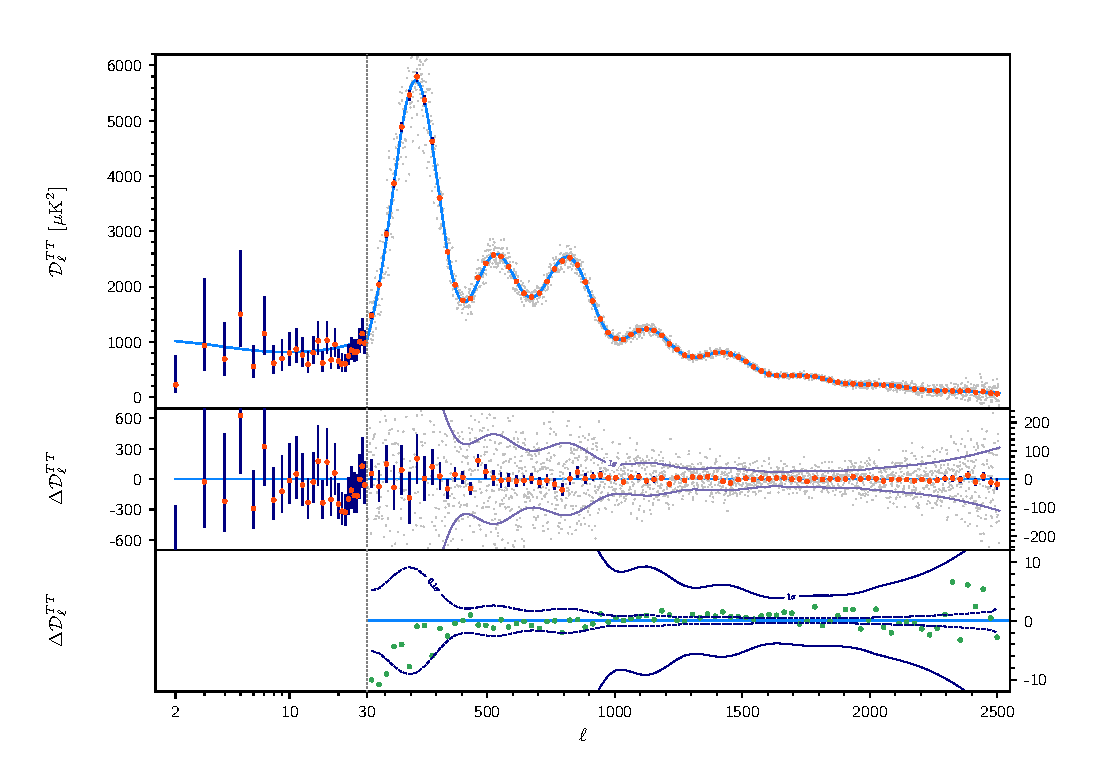
\includegraphics[width=0.99\linewidth]{figures/high_ell/TT_head_comp_2015}
		\caption{Planck 2018 temperature power spectrum.  The base-$\Lambda$CDM theoretical spectrum best fit to the likelihoods is plotted in light blue in the upper panel. Residuals with respect to this model are shown in the middle panel. The bottom panel displays the difference between the 2015 and 2018 coadded high-multipole spectra (green points). Source: \cite{Planck_2018_2020_V}}
		\label{fig:ttheadcomp2015}
	\end{figure}
	
	
	\section{Cosmic Chronometers (CC)}
	Using the differential age technique on massive, passively evolving galaxies, to calculate the time at which they were born \cite{Favale_2023}. This is based on the fact that the Hubble parameter, according to the FLRW metric, can be written as
	\begin{equation}
		H(z)=\frac{-1}{1+z}\frac{dz}{dt} \, ,
	\end{equation}
	where $dt/dz$ is the look-back time differential change with redshift. It is possible to estimate that derivative using the spectra of two ensembles of galaxies that formed at the same times, but with not identical redshifts, and thus calculating the Hubble parameter, if General Relativity (GR) is to be held valid. Other than that, however, the data is suitable to perform model-independent analyses, since is it not bound by any other cosmological assumption. The dataset of Cosmic Chronometers (CC) that we will use is compiled of 32 points on $H(z)$, and is listed in table \ref{CCH_DataSet} of appendix \ref{DataSets}.
	
	The $\chi^2$ function for CC is simply a diagonal covariance,
	\begin{equation}
		\chi^2_{CC}=\sum_{i=1}^{n}\frac{\left[ H_{\text{th}(z_i)} - H_\text{obs}(z_i) \right]^2}{\sigma^2_{H,i}} \, ,
	\end{equation}
	where $H_{\text{th}(z_i)}$ the theoretical value from $\Lambda$CDM (or any other model), and $\sigma^2_{H,i}$ the uncertainty of the measurement.
	
	\section{Type Ia Supernovae (SNIa)}
	A Type Ia supernova is a supernova that occurs in a binary system that consists of at least one white dwarf. Since white dwarfs have a fixed critical mass at which they explode, their peak luminosity is consistent, a trait that allows them to be used as \textit{standard candles}, meaning that, the visual magnitude of a type Ia supernova is an indicator of its distance from Earth.
	
	
	
	\section{Baryonic Acoustic Oscillations (BAO)}
	During the early Universe, the dense, primordial plasma gravitationally attracted matter towards it, while the heat of Compton scattering (photon-matter interactions) created outward pressure, causing oscillations similar to sound waves. These waves propagate in the coupled photon-baryon fluid of the pre-recombination era, and can be detected through Baryonic Acoustic Oscillations (BAO) \cite{Favale_2023, DESI:2025zgx, Alam_2017}, providing insight on the expansion of the Universe. Similar to SNIa, which are used as \textit{standard candles}, BAO are used as \textit{Standard Rulers}, since they represent a fixed distance in the Universe's history.
	
	The sound horizon $r_d$ in the pre-recombination era is the maximum comoving distance an acoustic wave can travel from the early Universe up until the "drag epoch" $z_d$, and can be calculated by the integral,
	\begin{equation}
		r_d=\int_{z_d}^{\infty}\frac{c_s(z)}{H(z)}dz \, , \quad z_d \approx 1060 \, .
	\end{equation}
	If we assume that standard physics is valid in the pre-recombination era, the scale of $r_d$ can be calculated by the CMB by the relation,
	\begin{equation}
		r_{d}=147.05\,\text{Mpc}\times \left(\frac{\omega_{b}}{0.02236}\right)^{-0.13}\left(\frac{\omega_{bc}}{0.1432}\right)^{-0.23}\left(\frac{N_{\text{eff}}}{3.04}\right)^{-0.1} \, ,
	\end{equation}
	where, $\omega_b=\Omega_b h^2$, $\omega_{bc}=(\Omega_b+\Omega_c)h^2$, the present fractional energy densities of baryonic and cold dark matter, and $h=H_0 /(100\text{km}s^{-1}\text{Mpc}^{-1})$. When we measure the \textit{standard ruler} $r_d$ at late-time redshift $z$, we constrain two components of the Universe's geometry:
	\begin{itemize}
		\item \textbf{Transverse Comoving Distance} $D_M$,
		\begin{equation}
			D_M(z)=\frac{1}{H_0 \sqrt{\Omega_k}}\sinh \left[ \sqrt{\Omega_k} \int_{0}^{z} \frac{dz'}{H(z')/H_0} \right] \, ,
		\end{equation} 
		which converges to the flat Universe,
		\begin{equation}
			D_M(z)=\frac{1}{H_0}\int_{0}^{z} \frac{dz'}{H(z')/H_0} \, .
		\end{equation}
		\item \textbf{Line of Sight Direction} $D_H$,
		\begin{equation}
			D_H(z)=\frac{1}{H(z)} \, .
		\end{equation}
	\end{itemize}
	The constrained quantities are then $D_M/r_d$ and $D_H/r_d$.
	
	We can then combine the CMB anisotropies, which provide constrains on $\omega_{b}$ and $\omega_{bc}$, with BAO, and calculate $r_d$, so as to measure accurately $D_M$ and $D_H$. The dataset of BAO measurements that we will use consists of 14 points and is listed in tables \ref{tab:BAO_DM_dimensionless}, \ref{tab:BAO_H_dimensionless} of appendix \ref{DataSets}. 
	
	\section{Redshift-Space Distortion (RSD)}
	Redshift-Space Distortion (RSD) is an effect in observational cosmology where the apparent distribution of galaxies is altered due to their peculiar velocities, separate from the expansion of the Universe. This can cause different types of effects based on the scale.
	\begin{itemize}
		\item The Small Scale "Fingers of God" effect, in which galaxies moving away from the Earth within the cluster, the Doppler effect makes them appear even further away, while for galaxies moving towards the Earth, it makes them appear closer. This causes a spherical cluster of galaxies to get stretched into a long "finger", pointing directly at the observer.
		\item The Large Scale "Kaiser" effect, in which galaxies on the near side of an overdensity look like the are moving away from the Earth, while galaxies on the far side look like the are moving towards the Earth. The result is that, visually, the overdensity of galaxies looks compressed along our line of sight. 
	\end{itemize}
	
	We define the parameter
	\begin{equation}
		f\sigma_8=\sigma(z)f(z) \, ,
	\end{equation}
	where $f(z)$ is the growth rate,
	\begin{equation}
		f(z)=-\frac{d \ln \delta(z)}{d \ln z} \, ,
	\end{equation}
	and $\sigma(z)$ the matter scattering amplitude,
	\begin{equation}
		\sigma(z)=\sigma_8 \frac{\delta(z)}{\delta(0)} \, .
	\end{equation}
	
	The dataset of RSD measurements that we will use consists of 7 points and is listed in tables \ref{tab:BAO_f8_final} of appendix \ref{DataSets}.
	
	\section{Problems that Rise from Observations - Cosmological Tensions}
	\subsection{The Hubble Constant Tension}
	The SH0ES collaboration maps out physical, geometric distances, independently from the $\Lambda$CDM model, using \textit{anchors}, which are parallax measurements and orbital mechanics to measure exact distances to nearby galaxies, \textit{calibrators} that calculate exactly how bright the stars in said galaxies are through Cepheid variables, and \textit{indicators}, which look for galaxies that contain both Cepheid stars and SNIa, and calibrate the absolute brightness of the Supernovae. These three components (rungs) build the \textit{Cosmic Distance Ladder} (CDL.) Direct measurements of the Universal expansion are listed in table \ref{tab:complete_distance_ladder}. 
	
	% =========================================================================
	% TABLE 1: COMPLETE DISTANCE LADDER-DEPENDENT MEASUREMENTS OF H0
	% =========================================================================
	\begin{table}[h!]
		\centering
		\scriptsize
		\begin{tabular}{llcl}
			\hline\hline
			First Author \& Year & $H_0$ Value [km s$^{-1}$ Mpc$^{-1}$] & $\sigma_{H_0}$ & Key Methodology / Calibrator \\ 
			\hline
			Riess et al. (2022) [SH0ES]   & 73.04 & $\pm$ 1.04 & Cepheids + SNe Ia \\
			Freedman et al. (2021) [CCHP] & 69.8  & $\pm$ 1.7  & TRGB + SNe Ia \\
			Anand et al. (2021)           & 71.5  & $\pm$ 1.8  & TRGB (EDD) + SNe Ia \\
			Scolnic et al. (2023)         & 73.22 & $\pm$ 2.06 & Pantheoplus, SH0ES anchors \\
			Huang et al. (2020)           & 72.4  & $\pm$ 3.3  & Mira Variables + SNe Ia \\
			Blakeslee et al. (2021)       & 73.3  & $\pm$ 3.1  & Surface Brightness Fluctuations (SBF) \\
			Khetan et al. (2021)          & 70.5  & $\pm$ 4.1  & SBF Calibration \\
			de Jaeger et al. (2020)       & 75.8  & $\pm$ 5.1  & Type II Supernovae \\
			Freedman (2024)               & 72.6  & $\pm$ 2.0  & JWST Combined (TRGB/JAGB/Cepheids) \\
			Lee et al. (2024)             & 67.8  & $\pm$ 2.7  & JAGB + SNe Ia \\
			Li et al. (2024)              & 74.7  & $\pm$ 3.1  & JAGB Calibration \\
			Kenworthy et al. (2022)       & 73.1  & $\pm$ 2.5  & Two-rung distance ladder \\
			Pesce et al. (2020)           & 73.9  & $\pm$ 3.0  & Megamaser physical distances \\
			Brout et al. (2022)           & 73.5  & $\pm$ 1.1  & Pantheon+ Sample Calibration \\
			Riess et al. (2021)           & 73.2  & $\pm$ 1.3  & Cepheid Calibration of SNe Ia \\
			Soltis et al. (2021)          & 72.1  & $\pm$ 2.0  & Gaia EDR3 Parallaxes \\
			Dhawan et al. (2020)          & 75.1  & $\pm$ 3.0  & NIR Type Ia Supernovae \\
			Burns et al. (2018)           & 73.2  & $\pm$ 2.3  & CSP-I SN Ia Sample \\
			Breuval et al. (2020)         & 72.8  & $\pm$ 2.7  & Galactic Cepheids Calibration \\
			Reid et al. (2019)            & 73.5  & $\pm$ 1.4  & LMC Cepheid Geometry Anchor \\
			\hline
			\textbf{Weighted Mean Baseline} & \textbf{72.8} & \textbf{$\pm$ 0.5} & \textbf{All 20 Probes Combined} \\
			\hline\hline
		\end{tabular}
		\normalsize
		\caption{Local universe determinations of the Hubble constant ($H_0$) structurally linked to the SH0ES calibration framework, showing tight clustering around a high expansion rate baseline. Source: \cite{perivolaropoulos2024hubbletensiondistanceladder}}
		\label{tab:complete_distance_ladder}
	\end{table}
	
	The Planck satellite works differently than the CDL, by taking high-precision photographs of the CMB. It is responsible for measuring the densities of matter and dark matter, and the sound horizon $r_d$ at the CMB, at $z\sim 1100$. After gathering the data from the early Universe, we plug them into the $\Lambda$CDM model, simulating the 13.8 billion years of history, and finally calculating the Hubble constant $H_0$. Several results from the Planck satellite are shown in table \ref{tab:complete_one_step}.
	
	% =========================================================================
	% TABLE 2: COMPLETE ONE-STEP MEASUREMENTS (DISTANCE LADDER INDEPENDENT)
	% =========================================================================
	\begin{table}[h!]
		\centering
		\scriptsize
		\begin{tabular}{llcl}
			\hline\hline
			First Author \& Year & $H_0$ Value [km s$^{-1}$ Mpc$^{-1}$] & $\sigma_{H_0}$ & Source Probe / Statistical Strategy \\ 
			\hline
			Moresco et al. (2022)         & 67.7  & $\pm$ 3.3  & Cosmic Chronometers ($d z/d t$) \\
			Borghi et al. (2022)          & 68.3  & $\pm$ 4.0  & Cosmic Chronometers, Stellar Ages \\
			Gomez-Valent et al. (2024)    & 69.5  & $\pm$ 2.5  & Sound-Horizon Free BAO + CC \\
			Simon et al. (2005)           & 69.0  & $\pm$ 12.0 & Baseline Cosmic Chronometers \\
			Zhang et al. (2014)           & 68.9  & $\pm$ 4.1  & Cosmic Chronometers \\
			Ratsimbazafy et al. (2017)    & 68.1  & $\pm$ 5.1  & CC, Faint Galaxy Populations \\
			Wong et al. (2020) [H0LiCOW]  & 73.3  & $\pm$ 1.8  & Strong Lensing Time-Delay \\
			Birrer et al. (2020)          & 67.4  & $\pm$ 4.1  & TDCOSMO, Model-Independent Lensing \\
			Shajib et al. (2023)          & 71.3  & $\pm$ 2.4  & Strong Lensing Cluster Analysis \\
			Kelly et al. (2023)           & 66.6  & $\pm$ 4.1  & Supernova Refsdal Time Delays \\
			Abbott et al. (2021)          & 68.0  & $^{+12.0}_{-7.0}$ & GW170817 Standard Siren (Direct) \\
			Sneppen et al. (2023)         & 75.5  & $\pm$ 4.1  & Kilonova Ejecta Geometry \\
			Barua et al. (2025)           & 69.1  & $\pm$ 2.1  & Megamaser Cosmology Project \\
			Dominguez et al. (2019)       & 67.4  & $^{+6.0}_{-6.2}$ & Gamma-ray Attenuation (BL Lacs) \\
			Boyle et al. (2023)           & 68.4  & $\pm$ 4.7  & X-ray Cluster Gas Mass Fractions \\
			Kozmanyan et al. (2019)       & 67.3  & $\pm$ 3.8  & Sunyaev-Zeldovich effect + Clusters \\
			Kim et al. (2020)             & 69.4  & $\pm$ 4.5  & H II Galaxies as standard candles \\
			Fernandez-Arenas (2018)       & 68.9  & $\pm$ 3.4  & Giant H II Regions \\
			Dux et al. (2024)             & 70.2  & $\pm$ 3.8  & Fast Radio Burst (FRB) Dispersion \\
			Macquart et al. (2020)        & 70.0  & $\pm$ 9.0  & FRB Macquart Relation \\
			Wu et al. (2022)              & 68.5  & $\pm$ 4.9  & Direct Megamaser Detections \\
			Pesce et al. (2020) [MCP]     & 73.9  & $\pm$ 3.0  & MCP Joint Assembly \\
			Gao et al. (2021)             & 69.2  & $\pm$ 4.2  & Gravitational Wave Host Studies \\
			Gayathri et al. (2023)        & 68.8  & $\pm$ 5.4  & Bright Siren Constellation \\
			Lusso et al. (2019)           & 67.5  & $\pm$ 5.2  & Quasar X-ray / UV Luminosity Relation \\
			Risaliti \& Lusso (2021)      & 68.0  & $\pm$ 4.0  & High-z Quasars Core Sample \\
			Dainotti et al. (2021)        & 69.5  & $\pm$ 3.5  & Gamma-Ray Burst (GRB) Correlations \\
			Cardone et al. (2018)         & 68.7  & $\pm$ 4.3  & Extended GRB Fundamental Plane \\
			Taylor et al. (2023)          & 68.9  & $\pm$ 2.4  & CC + Non-parametric Smoothing \\
			Favale et al. (2024)          & 68.2  & $\pm$ 1.9  & CC + Angular BAO Combos \\
			Scolnic et al. (2020)         & 68.1  & $\pm$ 4.5  & Spatial Void Dynamics \\
			Horinouchi et al. (2023)      & 69.0  & $\pm$ 3.6  & Super-luminous Supernovae \\
			Verde et al. (2019)           & 68.5  & $\pm$ 2.2  & Combined Standard One-Step Consensus \\
			\hline
			\textbf{Weighted Mean Baseline} & \textbf{69.0} & \textbf{$\pm$ 0.48} & \textbf{All 33 Probes Combined} \\
			\textbf{Excluding Outliers}     & \textbf{68.3} & \textbf{$\pm$ 0.50} & \textbf{Omitting TDCOSMO.I-2019 / High Outliers} \\
			\hline\hline
		\end{tabular}
		\normalsize
		\caption{Hubble constant determinations from distance-ladder-independent cosmic probes. The aggregated weighted mean aligns closely with the early-universe physics inferred by the Planck satellite. Source: \cite{perivolaropoulos2024hubbletensiondistanceladder}}
		\label{tab:complete_one_step}
	\end{table}
	
	We notice that the two tables follow two distinct distributions, leading to conflicting values of $H_0$. This clash leads two three possible scenarios:
	\begin{enumerate}
		\item SH0ES is not working as intended, and there is a systematic error in the ways through which we calibrate our machines,
		\item Planck is not plugging the raw data into the correct model, meaning that during that simulated fast-forward, the $\Lambda$CDM model shows unnoticed flaws, raising a need for new physics, or
		\item a combination of the above.
	\end{enumerate}
	
	\subsection{The $\sigma_8$ Tension}
	Another parameter that we calculate is $\sigma_8$, which is the rms amplitude of matter density fluctuations in spheres of comoving radius $8h^{-1}\text{Mpc}$, defined by the matter power spectrum $P(k)$,
	\begin{equation}
		\sigma_8^2=\int \frac{dk}{k} \frac{k^3 P(k)}{2\pi^2}W^2(kR) \, ,
	\end{equation}
	where $W$ a spherical top-hat function, and $R=8h^{-1}\text{Mpc}$, and represents how "lumpy" or smooth the Universe is at that scale. Weak lensing surveys are more sensitive to the combination
	\begin{equation}
		S_8\equiv\sigma_8\sqrt{\frac{\Omega_m}{0.3}} \, .
	\end{equation}
	Compiled $S_8$ measurements from various surveys are shown in fig. \ref{fig:s8_plot} and in table \ref{tab:s8_measurements}. As with the $H_0$ tensions, there is still a conflict between the theoretical models and the model-independent techniques, although not as high ($ \lesssim 3\sigma$).
	
	\begin{figure}[h]
		\begin{tikzpicture}
			\begin{axis}[
				width=0.92\textwidth,
				height=13cm,
				xlabel={Year of Publication},
				ylabel={$S_8 \equiv \sigma_8(\Omega_m/0.3)^{0.5}$},
				xmin=2019.0, xmax=2026.7,
				ymin=0.65, ymax=0.90,
				x tick label style={/pgf/number format/1000 sep=},
				xtick={2020, 2021, 2022, 2023, 2024, 2025, 2026},
				ytick={0.65, 0.68, 0.70, 0.72, 0.74, 0.76, 0.78, 0.80, 0.82, 0.84, 0.86, 0.88, 0.90},
				legend style={
					at={(0.98,0.02)},
					anchor=south east,
					font=\footnotesize,
					fill=white,
					fill opacity=0.95,
					draw=gray,
					cells={anchor=west},
					row sep=1pt,
					/tikz/every even column/.append style={column sep=5pt}
				},
				legend columns=1,
				grid=major,
				grid style={dashed, gray!30},
				clip=false
				]
				
				% Combined CMB Baseline (Gray Band) - asymmetric: 0.836 +0.012 / -0.013
				\addplot [name path=upper, draw=none, forget plot] coordinates {(2019.3, 0.848) (2026.7, 0.848)};
				\addplot [name path=lower, draw=none, forget plot] coordinates {(2019.3, 0.823) (2026.7, 0.823)};
				\addplot [gray!25, forget plot] fill between [of=upper and lower];
				\addplot [gray, thick, dashed, forget plot] coordinates {(2019.3, 0.836) (2026.7, 0.836)};
				\node[gray, anchor=south west, font=\footnotesize\bfseries, fill=white, fill opacity=0.8, inner sep=2pt] at (axis cs: 2024.5, 0.852) {Combined CMB $1\sigma$};
				
				% --- DATA POINTS (asymmetric error bars via table format) ---
				
				% CMB Points (Black squares) — all symmetric
				\addplot[only marks, mark=square*, mark size=3pt, color=black, 
				error bars/.cd, y dir=both, y explicit]
				table [x index=0, y index=1, y error plus index=2, y error minus index=3] {
					2020.0  0.832  0.013  0.013
					2025.8  0.875  0.023  0.023
					2026.0  0.828  0.012  0.012
				};
				\addlegendentry{CMB \& CMB Lensing}
				
				% DES Data (Red circles) — asymmetric errors
				\addplot[only marks, mark=*, mark size=3.5pt, color=red!85!black, 
				error bars/.cd, y dir=both, y explicit]
				table [x index=0, y index=1, y error plus index=2, y error minus index=3] {
					2022.1  0.776  0.017  0.017
					2024.2  0.823  0.019  0.020
					2026.0  0.794  0.009  0.012
					2026.1  0.789  0.012  0.012
					2026.2  0.783  0.019  0.015
					2026.3  0.781  0.021  0.020
					2026.5  0.747  0.027  0.025
				};
				\addlegendentry{Dark Energy Survey (DES)}
				
				% KiDS Data (Blue circles) — asymmetric errors
				\addplot[only marks, mark=*, mark size=3.5pt, color=blue!85!black, 
				error bars/.cd, y dir=both, y explicit]
				table [x index=0, y index=1, y error plus index=2, y error minus index=3] {
					2021.0  0.759  0.024  0.021
					2023.8  0.790  0.018  0.014
					2025.2  0.815  0.016  0.021
				};
				\addlegendentry{Kilo-Degree Survey (KiDS)}
				
				% Cluster Counts (Orange triangles) — all symmetric
				\addplot[only marks, mark=triangle*, mark size=4pt, color=orange!90!black, 
				error bars/.cd, y dir=both, y explicit]
				table [x index=0, y index=1, y error plus index=2, y error minus index=3] {
					2019.5  0.800  0.050  0.050
					2024.0  0.795  0.029  0.029
					2024.1  0.780  0.020  0.020
					2024.7  0.860  0.010  0.010
				};
				\addlegendentry{Galaxy Cluster Counts}
				
				% HSC (Green diamonds) — asymmetric errors
				\addplot[only marks, mark=diamond*, mark size=4pt, color=green!65!black, 
				error bars/.cd, y dir=both, y explicit]
				table [x index=0, y index=1, y error plus index=2, y error minus index=3] {
					2019.2  0.780  0.030  0.033
					2023.4  0.812  0.021  0.021
					2023.6  0.775  0.043  0.038
					2023.9  0.776  0.032  0.033
					2025.4  0.805  0.018  0.018
				};
				\addlegendentry{Hyper Suprime-Cam (HSC)}
				
				% Other probes (Purple pentagons) — some asymmetric
				\addplot[only marks, mark=pentagon*, mark size=3.5pt, color=purple!80!black, 
				error bars/.cd, y dir=both, y explicit]
				table [x index=0, y index=1, y error plus index=2, y error minus index=3] {
					2020.9  0.776  0.033  0.033
					2021.2  0.762  0.030  0.025
					2021.5  0.700  0.038  0.037
					2023.0  0.792  0.022  0.022
					2024.3  0.816  0.024  0.024
					2024.5  0.775  0.027  0.027
					2025.0  0.808  0.017  0.017
					2025.1  0.829  0.011  0.011
					2025.5  0.819  0.030  0.030
					2025.9  0.810  0.050  0.050
				};
				\addlegendentry{Other (DESI, RSD, GGL, Ly$\alpha$, Sat.\ Kin.)}
				
				% Key annotations
				\node[red!85!black, font=\scriptsize, anchor=north west] at (axis cs: 2026.2, 0.785) {DES Y6};
				\node[red!85!black, font=\scriptsize, anchor=north] at (axis cs: 2026.5, 0.740) {DES Y1};
				\node[red!85!black, font=\scriptsize, anchor=south east] at (axis cs: 2024.1, 0.825) {WL+kSZ};
				\node[blue!85!black, font=\scriptsize, anchor=south west] at (axis cs: 2025.3, 0.817) {KiDS};
				\node[orange!90!black, font=\scriptsize, anchor=south] at (axis cs: 2024.7, 0.875) {eROSITA};
				\node[black, font=\scriptsize, anchor=east] at (axis cs: 2019.9, 0.832) {Planck};
				\node[black, font=\scriptsize, anchor=west] at (axis cs: 2025.9, 0.880) {ACT DR6};
				\node[purple!80!black, font=\scriptsize, anchor=east] at (axis cs: 2021.4, 0.693) {Benisty};
				\node[purple!80!black, font=\scriptsize, anchor=east] at (axis cs: 2021.1, 0.755) {Nunes};
				
			\end{axis}
		\end{tikzpicture}
		\caption{Compilation of $S_8$ measurements from major cosmological surveys (2019--2026). The horizontal gray band represents the $1\sigma$ confidence interval of the Combined CMB baseline (Planck + ACT DR6 + SPT-3G), centered at $S_8 = 0.836$ with asymmetric width $^{+0.012}_{-0.013}$. The dashed gray line indicates the central value. Source: \cite{Pantos_2026}.}                                                                                                                                                                                                                                     
		\label{fig:s8_plot}
	\end{figure}                                                                                                                                                                                                                                                                                               

	
	\begin{table}[htbp]
		\centering
		\scriptsize % Reduces font size slightly to fit dense data comfortably on the page
		\begin{tabularx}{\textwidth}{lll c X} % 'X' stretches to perfectly fill the rest of the text width
			\hline\hline
			\textbf{Probe / Analysis} & \textbf{Date} & \textbf{$S_8$ Value} & \textbf{Tension} & \textbf{Reference \& Notes} \\ \hline
			
			\multicolumn{5}{l}{\textbf{CMB \& Early Universe Baselines}} \\ \hline
			Combined CMB & Jan 2026 & $0.836_{-0.013}^{+0.012}$ & — & Planck+ACT+SPT; primary baseline (Abbott et al., 2026) \\
			Combined Lensing & Jan 2026 & $0.828 \pm 0.012$ & $0.5\sigma$ & ACT+SPT+Planck lensing + DESI DR2 BAO (Qu et al., 2026) \\
			ACT DR6 (primary CMB) & Nov 2025 & $0.875 \pm 0.023$ & $-1.5\sigma$ & ACT DR6 power spectra alone (+ Sroll2 $\tau$ prior); above baseline (Louis et al., 2025) \\
			Planck 2018 & Sep 2020 & $0.832 \pm 0.013$ & — & Previous baseline (Planck Collaboration et al., 2020) \\ \hline
			
			\multicolumn{5}{l}{\textbf{Dark Energy Survey}} \\ \hline
			DES Y6 (All) & Jan 2026 & $0.794_{-0.012}^{+0.009}$ & $2.4\sigma$ & 3$\times$2pt + BAO + SNe + clusters (Abbott et al., 2026) \\
			DES Y6 ($3 \times 2$pt) & Jan 2026 & $0.789 \pm 0.012$ & $2.7\sigma$ & $3 \times 2$pt analysis (cosmic shear + galaxy clustering + galaxy-galaxy lensing) (Abbott et al., 2026) \\
			DES Y6 (Shear) & Jan 2026 & $0.783_{-0.015}^{+0.019}$ & $2.7\sigma$ & Cosmic shear only (Abbott et al., 2026) \\
			DES Y6 ($w$CDM) & Jan 2026 & $0.781_{-0.020}^{+0.021}$ & $1.0\sigma$ & Extended model; reported tension (projected) (Abbott et al., 2026) \\
			DES Y3 WL + ACT kSZ & Apr 2024 & $0.823_{-0.020}^{+0.019}$ & $0.6\sigma$ & Joint WL + kSZ with BCEmu7 baryonification (Bigwood et al., 2024) \\
			DES Y3 ($3 \times 2$pt) & Jan 2022 & $0.776 \pm 0.017$ & $2.8\sigma$ & Previous DES release (Abbott et al., 2022) \\
			DES Y1 ($3 \times 2$pt) & Jan 2026 & $0.747_{-0.025}^{+0.027}$ & $3.2\sigma$ & Reanalysis with Y6 pipeline (Abbott et al., 2026) \\ \hline
			
			\multicolumn{5}{l}{\textbf{Kilo-Degree Survey}} \\ \hline
			KiDS-Legacy (Shear) & Mar 2025 & $0.815_{-0.021}^{+0.016}$ & $0.9\sigma$ & Final KiDS result (Wright et al., 2025) \\
			KiDS-1000 + DES Y3 & Oct 2023 & $0.790_{-0.014}^{+0.018}$ & $2.4\sigma$ & Joint cosmic shear analysis (Abbott et al., 2023) \\
			KiDS-1000 (Shear) & Jan 2021 & $0.759_{-0.021}^{+0.024}$ & $3.1\sigma$ & Superseded (Asgari et al., 2021) \\ \hline
			
			\multicolumn{5}{l}{\textbf{Hyper Suprime-Cam}} \\ \hline
			HSC Y3 (DESI $n(z)$) & Nov 2025 & $0.805 \pm 0.018$ & $1.4\sigma$ & Reanalysis with DESI clustering-$z$ calibration (Choppin de Janvry et al., 2025) \\
			HSC Y3 ($3 \times 2$pt, minimal bias) & Dec 2023 & $0.775_{-0.038}^{+0.043}$ & $1.5\sigma$ & HSC shear + SDSS clustering (Sugiyama et al., 2023) \\
			HSC Y3 (Shear) & Dec 2023 & $0.776_{-0.033}^{+0.032}$ & $1.7\sigma$ & Third-year analysis (Dalal et al., 2023) \\
			HSC Y1 (Unified) & Apr 2023 & $0.812 \pm 0.021$ & $1.0\sigma$ & Unified pipeline (Longley et al., 2023) \\
			HSC Y1 (Original) & Mar 2019 & $0.780_{-0.033}^{+0.030}$ & $1.6\sigma$ & Original analysis (Hikage et al., 2019) \\ \hline
			
			\multicolumn{5}{l}{\textbf{Galaxy Cluster Counts}} \\ \hline
			eROSITA (X-ray) & Oct 2024 & $0.86 \pm 0.01$ & $-1.5\sigma$ & Higher than CMB (Ghirardini et al., 2024) \\
			SPT-3G Clusters & Jan 2024 & $0.795 \pm 0.029$ & $1.3\sigma$ & SZ-selected (Bocquet et al., 2024) \\
			Planck SZ (Chandra+WL) & Feb 2024 & $0.78 \pm 0.02$ & $2.3\sigma$ & PSZ2 cluster counts, Chandra X-ray + CFHT WL mass calibration; baseline self-similar model (Aymerich et al., 2024) \\
			Planck+CMB lensing & 2019 & $0.80 \pm 0.05$ & $0.7\sigma$ & Lensing mass calibration (Zubeldia and Challinor, 2019) \\ \hline
			
			\multicolumn{5}{l}{\textbf{Spectroscopic \& Other Probes}} \\ \hline
			Satellite Kinematics (SDSS) & Dec 2025 & $0.81 \pm 0.05$ & $0.5\sigma$ & Basilisk: sat. kinematics + luminosity function (Mitra et al., 2025) \\
			GGL (HSC$\times$BOSS) & Feb 2025 & $0.8294 \pm 0.0110$ & $0.4\sigma$ & Galaxy-galaxy lensing (Luo et al., 2025) \\
			DESI DR1 + Lensing & May 2025 & $0.808 \pm 0.017$ & $1.3\sigma$ & 3D clustering + CMB lensing (Maus et al., 2025) \\
			Peculiar Velocities & Sep 2025 & $0.819 \pm 0.030$ & $0.5\sigma$ & TFR+FP+SNe joint (Stiskalek, 2025) \\
			BOSS$\times$DECaLS (Magnification) & Sep 2024 & $0.816 \pm 0.024$ & $0.7\sigma$ & Lensing magnification of CMASS galaxies (Xu et al., 2024) \\
			RSD compilation & Aug 2024 & $0.775 \pm 0.027$ & $2.0\sigma$ & RSD+DESI+PP (Sabogal et al., 2024) \\
			BOSS Full-Shape & 2023 & $0.792 \pm 0.022$ & $1.7\sigma$ & Clustering + GGL (Lange et al., 2023) \\
			RSD (Benisty) & 2021 & $0.700_{-0.037}^{+0.038}$ & $3.5\sigma$ & RSD compilation (Benisty, 2021) \\
			RSD+BAO+SNe & 2021 & $0.762_{-0.025}^{+0.030}$ & $2.6\sigma$ & RSD compilation + BAO + SNeIa (Nunes and Vagnozzi, 2021) \\
			Ly$\alpha$ Forest & Nov 2020 & $0.776 \pm 0.033$ & $1.7\sigma$ & SDSS DR14 (Palanque-Delabrouille et al., 2020) \\ \hline\hline
			
		\end{tabularx}
		\normalsize
		
		\caption{Comprehensive compilation of $S_8$ measurements and their tension with the Combined CMB baseline ($S_8 = 0.836_{-0.013}^{+0.012}$). Tensions are computed using the uncertainty in the direction of the discrepancy for asymmetric errors. Negative values indicate $S_8$ above the baseline. Source: \cite{Pantos_2026}} 
		\label{tab:s8_measurements}
	\end{table}
	
	
	\chapter{Parameterizations of the $\Lambda$CDM Model}
	\section{The $w$CDM Model}
	The equation of state parameter is defined as
	\begin{equation}
		w_i\equiv\frac{p_i}{\rho_i} \, ,
	\end{equation}
	where $i$ denotes the type of matter. In the $w$CDM model \cite{sammut2025testingplanck2020desi}, dark energy does not take the role of a constant, and its density is calculated as
	\begin{equation}
		\rho_\Lambda=\rho_{\Lambda_0}a^{-3}\exp\left( -3 \int_{1}^{a} \frac{w_\Lambda(a')}{a'} da' \right) \, .
	\end{equation}
	Thus, the Friedmann equation for the wCDM model becomes
	\begin{equation}
		\label{wCDM_Friedmann_equation}
		H^2=\frac{8\pi G}{3}\left[ \rho_{r_0} a^{-4} + (\rho_{b_0} + \rho_{c_0})a^{-3} + =\rho_{\Lambda_0}a^{-3}\exp\left( -3 \int_{1}^{a} \frac{w_\Lambda(a')}{a'} da' \right) \right] \, .
	\end{equation}
	From this metric, the perturbed continuity and Euler equations are derived,
	\begin{equation}
		\begin{array}{c}
			\delta'_i = -(1+w_i)\left( \theta_i + \frac{h'}{2} \right) - 3\mathcal{H} (c^2_s - w_i)\delta_i 9\mathcal{H}^2\left( \frac{\delta P_i}{\delta \rho_i} - c^2_{a,i} \right) (1+w_i)\frac{\theta_i}{k^2} \, , \\ \, \\ 
			\theta'_i=-\mathcal{H}\left( 1-3\frac{\delta P_i}{\delta \rho_i}  \right)\theta_i +\frac{\delta P_i}{\delta \rho_i} \frac{1}{1-w_i}k^2 \delta_i-k^2\sigma_i \, ,
		\end{array}
	\end{equation}
	where $h=$ the trace of the metric perturbations, $\theta_i\equiv ik^j v_j$ the divergence of the $i$th fluid, $c^2_s$ the sound speed of an imperfect fluid, $\sigma_i$ the anisotropic stress of the fluid,	and $c^2_{a,i}$ the adiabatic sound speed
	\begin{equation}
		c^2_{a,i}=w_i-\frac{w'_i}{3\mathcal{H}(1+w'_i)} \, .
	\end{equation}
	Below we showcase different parameterization scenarios along with their properties.
	\begin{enumerate}
		\item \textbf{The $w_0$CDM Parameterization}
		
		In the $w_0$CDM model, we deviate from the $\Lambda$CDM model, by assigning a constant value that is unequal to $-1$. Thus, we write $w(a)$ as
		\begin{equation}
			w_{w\text{CDM}}(a)=w_{w_0\text{CDM}}\neq -1 \, ,
		\end{equation}
		and we call this the constant $w$CDM model.
		\item \textbf{The JBP Parameterization}
		
		We use a non-linear dynamical dark energy equation, writing $w(a)$ as
		\begin{equation}
			w_{w\text{CDM}}(a)=w_{w_0\text{JBO}}+w_{w_a\text{JBP}}a(1-a) \, ,
		\end{equation}
		which was suggested by Jassal-Bagla-Padmanabhan.
		\item \textbf{The GE (Logarithmic) Model}
		
		We use a logarithmic dark energy equation,
		\begin{equation}
			w_{w\text{CDM}}(a)=w_{w_0\text{GE}-w_{w_a\text{GE}}}\ln(a) \, ,
		\end{equation}
		which was proposed by G. Efstathiou.
		\item \textbf{The Oscillatory Model}
		
		We use an oscillatory equation state for dark energy,
		\begin{equation}
			w_{w\text{CDM}}(a)=w_{0\text{OSC}}+w_{a\text{OSC}}\left[ a\sin\left(\frac{1}{a}\right)\right] \, .
		\end{equation}
	\end{enumerate}

	\section{The Hubble Function Parameterization}
	A generalization of the $w_0$CDM model is the parameterization of the Hubble function into the form
	\begin{equation}
		H^2=H^2_0\left[ \Omega_0(1+z)^{3+\delta} + (1-\Omega_0)(1+z)^\alpha \right]\, ,
	\end{equation}
	where $\Omega_0,\,\delta,\,\alpha$ are constants that mimic the $\Lambda$CDM equivalent equation for $(\delta,\alpha)=(0,0)$, with the only difference being the parameter $\Omega_0$. In this case, $\Omega_0$ may not correspond to the density parameter $\Omega_{m0}$ due to possibly including the density parameters of other participating fluids. Using this parameterization, we can interpret each term as a non-interacting fluid, such as a Dark Matter-like (DM-like) fluid and Dark Energy (DE), through which we notice that DM is not purely cold, and has an equation of state (EoS) $\delta/3$, while DE has an EoS $w=-1+\alpha/3$. In this case $\Omega_{0}$ does correspond closely to $\Omega_{m0}$, however this is not a necessary condition for our model. We can also rewrite is as,
	\begin{equation}
		H^2=H^2_0 \left\{ \underbrace{ \left[ \Omega_0(1+z)^{3+\delta} +g(z) \right]}_{\tilde{\Omega}_1} + \underbrace{ \left[ (1-\Omega_0)(1+z)^\alpha-g(z) \right]}_{\tilde{\Omega}_2} \right\}= H^2_0\left[ \tilde{\Omega}_1 + \tilde{\Omega}_2 \right] \, ,
	\end{equation} 
	where, $\tilde{\Omega}_i \equiv \rho_i/\rho_{c0}$, where $\rho_i$ the energy density of each fluid, and $\rho_{c0}$ the critical energy density. 
	
	If the two fluids are not interacting with each other, we can write the two separate conservation equation for each one,
	\begin{equation}
			\dot \rho_i + 3H(1+w_i)\rho_i=0 \, , 
	\end{equation}
	and by writing $w_i$ as
	\begin{equation}
		w_i=-1-\frac{\alpha}{3\rho_i}\cdot \frac{d\rho_i}{da}=-1-\frac{1}{3\tilde{\Omega}_i}\frac{\tilde{d \Omega}_i}{da}\, ,
	\end{equation}
	we can easily calculate the EoS parameters for specific functions $g(a)$.
	
	If the two fluids are interacting, then we write the conservation equation as
	\begin{equation}
		\begin{array}{c}
			\frac{d\rho_1}{dt}+3H(1+w_1)\rho_1=-Q \, , \\ \, \\
			\frac{d\rho_2}{dt}+3H(1+w_2)\rho_2=+Q \, ,
		\end{array}
	\end{equation}
	where $Q$ the interaction term. If we plug the expressions of $\rho_1$, $\rho_2$ into the above equations, we can write
	\begin{equation}
		g(a)=\left( \frac{\delta/3-w_1}{w_1-w_2} \right) \Omega_0 a^{-(3+\delta)}- \left( \frac{1+w_2-\alpha/3}{w_1-w_2} \right) (1-\Omega_0)a^{-\alpha} = A\Omega_0 a^{-(3+\delta)}-B(1-\Omega_0)a^{-\alpha} \, . 
	\end{equation}
	
	\chapter{Theories of Modified Gravity}
	
	\appendix
	\chapter{Data Sets}
	\label{DataSets}
	\section{Cosmic Chronometer Dataset}
	Hubble parameter measurements from DR2 \cite{DESI:2025zgx}.
	\begin{table}[h!]
		\centering
		\small
		\begin{tabular}{ccc}
			\hline\hline
			$z$ & $H(z)$ [km/s/Mpc] & References \\ \hline
			0.07 & $69.0 \pm 19.6$ & Zhang et al. (2014) \\
			0.09 & $69.0 \pm 12.0$ & Jimenez et al. (2003) \\
			0.12 & $68.6 \pm 26.2$ & Zhang et al. (2014) \\
			0.17 & $83.0 \pm 8.0$ & Simon et al. (2005) \\
			0.1791 & $78.0 \pm 6.2$ & Moresco et al. (2012) \\
			0.1993 & $78.0 \pm 6.9$ & Moresco et al. (2012) \\
			0.2 & $72.9 \pm 29.6$ & Zhang et al. (2014) \\
			0.27 & $77.0 \pm 14.0$ & Simon et al. (2005) \\
			0.28 & $88.8 \pm 36.6$ & Zhang et al. (2014) \\
			0.3519 & $85.5 \pm 15.7$ & Moresco et al. (2012) \\
			0.3802 & $86.2 \pm 14.6$ & Moresco et al. (2016) \\
			0.4 & $95.0 \pm 17.0$ & Simon et al. (2005) \\
			0.4004 & $79.9 \pm 11.4$ & Moresco et al. (2016) \\
			0.4247 & $90.4 \pm 12.8$ & Moresco et al. (2016) \\
			0.4497 & $96.3 \pm 14.4$ & Moresco et al. (2016) \\
			0.47 & $89.0 \pm 49.6$ & Ratsimbazafy et al. (2017) \\
			0.4783 & $83.8 \pm 10.2$ & Moresco et al. (2016) \\
			0.48 & $97.0 \pm 62.0$ & Stern et al. (2010) \\
			0.5929 & $107.0 \pm 15.5$ & Moresco et al. (2012) \\
			0.6797 & $95.0 \pm 10.5$ & Moresco et al. (2012) \\
			0.75 & $98.8 \pm 33.6$ & Borghi et al. (2022) \\
			0.7812 & $96.5 \pm 12.5$ & Moresco et al. (2012) \\
			0.8754 & $124.5 \pm 17.4$ & Moresco et al. (2012) \\
			0.88 & $90.0 \pm 40.0$ & Stern et al. (2010) \\
			0.9 & $117.0 \pm 23.0$ & Simon et al. (2005) \\
			1.037 & $133.5 \pm 17.6$ & Moresco et al. (2012) \\
			1.3 & $168.0 \pm 17.0$ & Simon et al. (2005) \\
			1.363 & $160.0 \pm 33.8$ & Moresco (2015) \\
			1.43 & $177.0 \pm 18.0$ & Simon et al. (2005) \\
			1.53 & $140.0 \pm 14.0$ & Simon et al. (2005) \\
			1.75 & $202.0 \pm 40.0$ & Simon et al. (2005) \\
			1.965 & $186.5 \pm 50.6$ & Moresco (2015) \\ \hline\hline
		\end{tabular}
		\normalsize
		\caption{Cosmic Chronometer Data Pairs}
		\label{CCH_DataSet}
	\end{table}
	
	\section{Baryonic Acoustic Oscillations}
	BAO measurements from DR2 \cite{DESI:2025zgx}, DR12 \cite{Alam_2017} and DR14 \cite{Zhao_2018}.
	% ==========================================
	% TABLE 1: Unified Dimensionless Transverse Comoving Distance (D_M / r_d)
	% ==========================================
	\begin{table}[h!]
		\centering
		\footnotesize
		\begin{tabular}{cccccc}
			\hline\hline
			Data Sample / Tracer & Redshift ($z$) & BAO-only ($D_M/r_d$) & Full-shape ($D_M/r_d$) & Joint Consensus ($D_M/r_d$) \\ \hline
			DESI DR2 (BGS)        & $z = 0.295$ & — & — & — \\
			BOSS DR12             & $z = 0.38$  & $10.23 \pm 0.15 \pm 0.07$ & $10.35 \pm 0.16 \pm 0.07$ & $10.27 \pm 0.14 \pm 0.07$ \\
			BOSS DR12             & $z = 0.51$  & $13.36 \pm 0.18 \pm 0.09$ & $13.58 \pm 0.20 \pm 0.10$ & $13.38 \pm 0.16 \pm 0.09$ \\
			DESI DR2 (LRG1)       & $z = 0.510$ & — & — & $13.59 \pm 0.17$ \\
			BOSS DR12             & $z = 0.61$  & $15.61 \pm 0.22 \pm 0.12$ & $15.39 \pm 0.24 \pm 0.12$ & $15.45 \pm 0.19 \pm 0.11$ \\
			DESI DR2 (LRG2)       & $z = 0.706$ & — & — & $17.35 \pm 0.18$ \\
			DESI DR2 (LRG3+ELG1)  & $z = 0.934$ & — & — & $21.58 \pm 0.15$ \\
			eBOSS DR14            & $z = 0.978$ & — & — & $21.59 \pm 3.89$ \\
			eBOSS DR14            & $z = 1.230$ & — & — & $26.00 \pm 2.36$ \\
			DESI DR2 (ELG2)       & $z = 1.321$ & — & — & $27.60 \pm 0.32$ \\
			DESI DR2 (QSO)        & $z = 1.484$ & — & — & $30.51 \pm 0.76$ \\
			eBOSS DR14            & $z = 1.526$ & — & — & $30.34 \pm 1.66$ \\
			eBOSS DR14            & $z = 1.944$ & — & — & $36.86 \pm 2.97$ \\
			DESI DR2 (Ly$\alpha$) & $z = 2.330$ & — & — & $38.99 \pm 0.53$ \\ \hline\hline
		\end{tabular}
		\normalsize
		\caption{Unified Dimensionless Constraints for the Transverse Comoving Distance Ratio $D_M(z)/r_d$}
		\label{tab:BAO_DM_dimensionless}
	\end{table}
	
	% ==========================================
	% TABLE 2: Unified Dimensionless Radial Hubble Distance (D_H / r_d)
	% ==========================================
	\begin{table}[h!]
		\centering
		\footnotesize
		\begin{tabular}{cccccc}
			\hline\hline
			Data Sample / Tracer & Redshift ($z$) & BAO-only ($D_H/r_d$) & Full-shape ($D_H/r_d$) & Joint Consensus ($D_H/r_d$) \\ \hline
			DESI DR2 (BGS)        & $z = 0.295$ & — & — & — \\
			BOSS DR12             & $z = 0.38$  & $24.98 \pm 0.68 \pm 0.31$ & $24.98 \pm 0.62 \pm 0.31$ & $24.89 \pm 0.52 \pm 0.28$ \\
			BOSS DR12             & $z = 0.51$  & $22.32 \pm 0.52 \pm 0.27$ & $22.98 \pm 0.55 \pm 0.26$ & $22.42 \pm 0.42 \pm 0.25$ \\
			DESI DR2 (LRG1)       & $z = 0.510$ & — & — & $21.86 \pm 0.43$ \\
			BOSS DR12             & $z = 0.61$  & $20.49 \pm 0.46 \pm 0.25$ & $21.22 \pm 0.53 \pm 0.24$ & $20.85 \pm 0.39 \pm 0.24$ \\
			DESI DR2 (LRG2)       & $z = 0.706$ & — & — & $19.46 \pm 0.33$ \\
			DESI DR2 (LRG3+ELG1)  & $z = 0.934$ & — & — & $17.64 \pm 0.19$ \\
			eBOSS DR14            & $z = 0.978$ & — & — & $19.34 \pm 2.38$ \\
			eBOSS DR14            & $z = 1.230$ & — & — & $17.21 \pm 1.63$ \\
			DESI DR2 (ELG2)       & $z = 1.321$ & — & — & $14.18 \pm 0.22$ \\
			DESI DR2 (QSO)        & $z = 1.484$ & — & — & $12.82 \pm 0.52$ \\
			eBOSS DR14            & $z = 1.526$ & — & — & $15.20 \pm 1.31$ \\
			eBOSS DR14            & $z = 1.944$ & — & — & $12.57 \pm 1.01$ \\
			DESI DR2 (Ly$\alpha$) & $z = 2.330$ & — & — & $8.63 \pm 0.10$ \\ \hline\hline
		\end{tabular}
		\normalsize
		\caption{Unified Dimensionless Constraints for the Radial Hubble Distance Ratio $D_H(z)/r_d$}
		\label{tab:BAO_H_dimensionless}
	\end{table}
	\section{Redshift-Space Distortion}
	BAO measurements from DR12 \cite{Alam_2017} and DR14 \cite{Zhao_2018}.
	% ==========================================
	% TABLE 3: Structure Growth Rate (f\sigma_8) [Kept for Completeness]
	% ==========================================
	\begin{table}[h!]
		\centering
		\footnotesize
		\begin{tabular}{cccccc}
			\hline\hline
			Data Sample / Tracer & Redshift ($z$) & BAO-only & Full-shape & Joint Consensus / Measured Value \\ \hline
			BOSS DR12   & $z = 0.38$  & — & $0.502 \pm 0.041 \pm 0.024$ & $0.497 \pm 0.039 \pm 0.024$ \\
			BOSS DR12   & $z = 0.51$  & — & $0.459 \pm 0.037 \pm 0.015$ & $0.458 \pm 0.035 \pm 0.015$ \\
			BOSS DR12   & $z = 0.61$  & — & $0.419 \pm 0.036 \pm 0.009$ & $0.436 \pm 0.034 \pm 0.009$ \\
			eBOSS DR14  & $z = 0.978$ & — & — & $0.379 \pm 0.176$ \\
			eBOSS DR14  & $z = 1.230$ & — & — & $0.383 \pm 0.086$ \\
			eBOSS DR14  & $z = 1.526$ & — & — & $0.407 \pm 0.054$ \\
			eBOSS DR14  & $z = 1.944$ & — & — & $0.435 \pm 0.053$ \\ \hline\hline
		\end{tabular}
		\normalsize
		\caption{Combined Constraints for the Structure Growth Rate Parameter $f(z)\sigma_8(z)$}
		\label{tab:BAO_f8_final}
	\end{table}
	
	\chapter{List of Tables}
	\chapter{List of Figures}
	
	\bibliographystyle{unsrtnat} % Or 'alpha', 'unsrt', etc.
	\bibliography{bibliography} % Points to your bibliography.bib file (leave off the .bib)
		

	
\end{document}
